\documentclass{ctuthesis}
\usepackage{graphicx}
\usepackage{lipsum}    
\usepackage{floatrow}
\usepackage{xargs}
\usepackage{setspace}                     
\usepackage[pdftex,dvipsnames,usenames,nonamebreak]{xcolor}
\usepackage[colorinlistoftodos,prependcaption,textsize=tiny]{todonotes}
\newcommandx{\unsure}[2][1=]{\todo[linecolor=red,backgroundcolor=red!25,bordercolor=red,#1]{#2}}
\newcommandx{\change}[2][1=]{\todo[linecolor=blue,backgroundcolor=blue!25,bordercolor=blue,#1]{#2}}
\newcommandx{\info}[2][1=]{\todo[linecolor=OliveGreen,backgroundcolor=OliveGreen!25,bordercolor=OliveGreen,#1]{#2}}
\newcommandx{\improvement}[2][1=]{\todo[linecolor=Plum,backgroundcolor=Plum!25,bordercolor=Plum,#1]{#2}}
\newcommandx{\thiswillnotshow}[2][1=]{\todo[disable,#1]{#2}}

\def\justifying{%
	\rightskip=0pt
	\spaceskip=0pt
	\xspaceskip=0pt
	\relax
}


\usepackage{subfig}
\usepackage{multicol}
\usepackage{tcolorbox}
\usepackage{tabularx}
\usepackage{array}
\usepackage{tikz}
\usepackage{fontawesome5}
\def\checkmark{\tikz\fill[scale=0.4](0,.35) -- (.25,0) -- (1,.7) -- (.25,.15) -- cycle;}
\usepackage{colortbl}
\tcbuselibrary{skins}
%\newcolumntype{Y}{>{\raggedleft\arraybackslash}X}
\tcbset{tab2/.style={enhanced,fonttitle=\bfseries,fontupper=\normalsize\sffamily,
		colback=yellow!10!white,colframe=red!50!black,colbacktitle=Salmon!40!white,
		coltitle=black,center title}}
	



%\usepackage{csquotes}
%\renewcommand*{\labelalphaothers}{}



\ctusetup{
	xdoctype = B,
	xfaculty = FCEyN,
	mainlanguage = czech,
	titlelanguage = czech,
	title-english = {},
	title-czech = {Construcción e implementación de un sistema integral de 
		caracterización de filtros ópticos utilizados en 
		cámaras 
		hiperespectrales.},
	department-czech = {Departamento de Física},
	author = {Juan Reto Reynal},
	supervisor = {Prof. Dr. Hernán Grecco},
	supervisor-address = {Laboratorio de Electrónica Cuántica, DF, FCEyN, UBA.},
	month = 4,
	year = 2020,
}


\ctuprocess





\def\ctucaptionsenglish{
	\def\appendicesname{Appendices}
	\def\thanksname{Carátula}
	\def\abstractname{Abstract}
	\def\declarationname{}
	\def\listfigurename{Figures}
	\def\listtablename{Tables}
	\def\supervisorname{Supervisor}
	\def\supervisorspecialistname{Supervisor--specialist}
	\def\fieldofstudyname{Field\ of\ study}
	\def\subfieldofstudyname{Subfield}
	\def\specificationname{Project\ Specification}
	\def\keywordsname{Keywords}
	\def\titletranslationname{Title\ translation}
}

\def\ctucaptionsczech{
	\def\appendicesname{Apéndice}
	\def\thanksname{}
	\def\contentsname{Índice}
	\def\abstractname{Resumen}
	\def\declarationname{}
	\def\listfigurename{Índice de Figuras}
	\def\listtablename{Índice de Tablas}
	\def\supervisorname{Director}
	\def\supervisorspecialistname{\v Skolitel--specialista}
	\def\fieldofstudyname{Obor}
	\def\subfieldofstudyname{Zam\v e\v ren\'i}
	\def\specificationname{Zad\'an\'i\ pr\'ace}
	\def\keywordsname{Palabras clave}
	\def\titletranslationname{P\v reklad\ n\'azvu}
}
%\newcommand\Chapter[2]{\chapter[#1:{\itshape#2}]{#1\\[2ex]\Large\itshape#2}}
\newcommand\Chapter[2]{\chapter[#1]{#1\\[1ex]\large#2}}

\begin{thanks}
	
	\raggedright
	\textsc{TEMA:} Construcción e implementación de un sistema integral de caracterización de filtros
	
	 \hspace{1.6cm}ópticos utilizados en cámaras hiperespectrales.
	
	\bigskip
	
	\textsc{ALUMNO:} Juan Reto Reynal
	
	\bigskip
	
	\textsc{L.U. N$^{\circ}$:} 777/12
	
	\bigskip
	
	\textsc{LUGAR DE TRABAJO:} LEC, Departamento de Física, FCEyN, UBA.
	
	
	\bigskip
	
	\textsc{DIRECTOR DEL TRABAJO:} Dr. Hernán E. Grecco
	
	\bigskip
	
	\textsc{FECHA DE INICIACIÓN:} Abril de 2019
	
	\bigskip
	
	\textsc{FECHA DE FINALIZACIÓN:} Abril de 2020
	
	\bigskip
	
	{\large FECHA DE EXAMEN: }
	
	\bigskip
	
	\textsc{INFORME FINAL APROBADO POR:}
	\vspace{2cm}
	
	\begin{center}
		\begin{tabular}{lll}
			\cline{1-1}\cline{1-1}\cline{3-3}\cline{3-3}%
			Autor:  & \hspace{2cm} & Jurado\ \ \ \ \ \ \ \ \ \ \ \ \ \ \
			\ \ \ \ \ \ \ \ \ \ \ \ \ \ \ \  \\
			&& \\
			&& \\
			&& \\
			\cline{1-1}\cline{1-1}\cline{3-3}\cline{3-3}%
			Director: \ \ \ \ \ \ \ \ \ \ \ \ \  & \hspace{2cm} & Jurado\\
			&& \\
			&& \\
			&& \\
			\cline{1-1}\cline{1-1}\cline{3-3}\cline{3-3}%
			Profesor: Juan Pablo Paz  & \hspace{2cm} & Jurado\\
			&& \\
			&& \\
			&& \\
		\end{tabular}	
	\end{center}
\justifying
\end{thanks}

\begin{declaration}

	Resumen copado al final..
	
	dkfjakdj
\end{declaration}



\begin{document}

\maketitle

\renewcommand{\chaptername}{Capítulo}
\renewcommand{\figurename}{Figura}


\setlength{\parindent}{0.5cm}
\setlength{\parskip}{1em}




\chapter{Introducción}
QUÉ ES UN DEFECTO Y QUÉ LE ESTÁ HACIENDO A LAS IMÁGENES, MOSTRAR IMAGEN QUE TIENE PUNTOS CON DIFRACCIÓN, LOS TIFFS..

\textsc{Título:} Construcción e implementación de un sistema integral de 
caracterización de filtros ópticos utilizados en cámaras hiperespectrales.


\hspace{-0.4cm}\textsc{Alumno:} Juan Reto Reynal L.U. 777/12.

\hspace{-0.4cm}\textsc{Director:} Dr. Hernán E. Grecco, 
Prof. Adj. UBA, Inv. Indep. CONICET.

\hspace{-0.4cm}\textsc{Lugar de trabajo:} LEC, Departamento de Física, FCEyN, UBA.


\section*{Objetivo general}
\hspace{0.5cm}La espectroscopía de imágenes hiperespectrales, en inglés 
\textit{Hyperspectral 
Spectroscopy Imaging} (HSI), combina la espectroscopía y la adquisición de 
imágenes 
en dos dimensiones. Este método brinda datos espectrales para cada 
pixel en el campo de 
visión\footnote{El campo de visión, en inglés \textit{field of view} (FOV), es 
el ángulo sólido a través del cual un sensor puede detectar la radiación 
electromagnética que se desee capturar.}. A partir de dichos 
datos se puede extraer información sobre la emisión, reflexión ó absorción de 
una muestra, que puede ser utilizada para determinar su 
composición físico-química con una resolución espacial. De esta forma se pueden 
identificar tumores de un cáncer, realizar un control de calidad de la comida 
identificando bacterias en tiempo real, localizar las células de una muestra 
biológica u optimizar la siembra y la cosecha de ciertos cultivos, entre otras 
aplicaciones.


En la tesis de licenciatura de Agustina Pose \cite{Pose2017}, dirigida 
por 
Hernán Grecco quien también dirige esta tesis, ambos desarrollaron un prototipo 
de cámara hiperespectral para uso satelital junto a la empresa Satellogic. Tras 
la realización de pruebas y mediciones en tierra, se aprobó la 
prueba de concepto de este prototipo y se lo adaptó a un diseño robusto. La 
cámara hiperespectral diseñada es hoy una de las cargas útiles (o 
\textit{payloads}) a bordo de los satélites argentinos NewSat 1 y NewSat 2 
(alias Fresco y Batata), puestos en órbita el 30 de Mayo de 2016, construidos 
por la empresa Satellogic.

En el presente proyecto se propone continuar con dicho trabajo y desarrollar un 
sistema integral de caracterización de los filtros de interferencia de banda 
que son utilizados en las cámaras hiperespectrales. Estos filtros permiten el 
paso de las longitudes de onda (colores) que se desean capturar con el sensor 
de detección principal de la cámara que sólo detecta intensidad lumínica, como 
se explica en la Introducción. En consecuencia, la caracterización de los 
filtros resulta fundamental para garantizar la calidad de las imágenes 
capturadas. El primer prototipo de este sistema integral permitirá 
principalmente caracterizar el espectro de transmisión del filtro en 
cada punto del mismo, es decir en cada posición $(x,y)$ de su superficie, y 
encontrar defectos que pudieran modificar su capacidad de bloqueo de ciertas 
longitudes de onda no deseadas.

\subsection*{Objetivos específicos del proyecto}
\begin{itemize}
	
	\item \texttt{Objetivo 1:} Caracterización de los espectros de transmisión 
	de los filtros.
	\item \texttt{Objetivo 2:} Detección de los defectos de los filtros 
	(\textit{scratch and dig}).
	\item \texttt{Objetivo 3:} Caracterización de los filtros en su posición 
	final en las cámaras de vuelo 
	del satélite. \end{itemize}
\section*{Introducción}

\hspace{0.5cm}Una imagen a color RGB convencional está compuesta por tres 
canales de 
imágenes (bandas): rojo 
($\sim$ 665nm), verde ($\sim$ 550nm) y azul ($\sim$ 470nm). Este tipo de 
imágenes permiten emular la percepción que el ojo humano tiene del color, pero 
en general no permiten la detección e identificación de distintos objetos 
sólidos y 
líquidos, menos 
aún determinar sus propiedades. Para ello 
es necesario obtener el espectro completo del objeto de estudio que es posible 
a partir de la captura de imágenes multiespectrales e hiperespectrales.

Las imágenes multiespectrales contienen un número acotado de bandas espectrales 
de hasta un par de decenas, con un gran ancho de banda (varias decenas de nm); 
mientras que las hiperespectrales están formadas por un gran número de bandas 
espectrales (de cientos a miles), con una resolución espectral muy estrecha, de 
unos pocos nm (Ver Figura \ref{fig:spectrus}).


\begin{figure}[H]
	\centering
	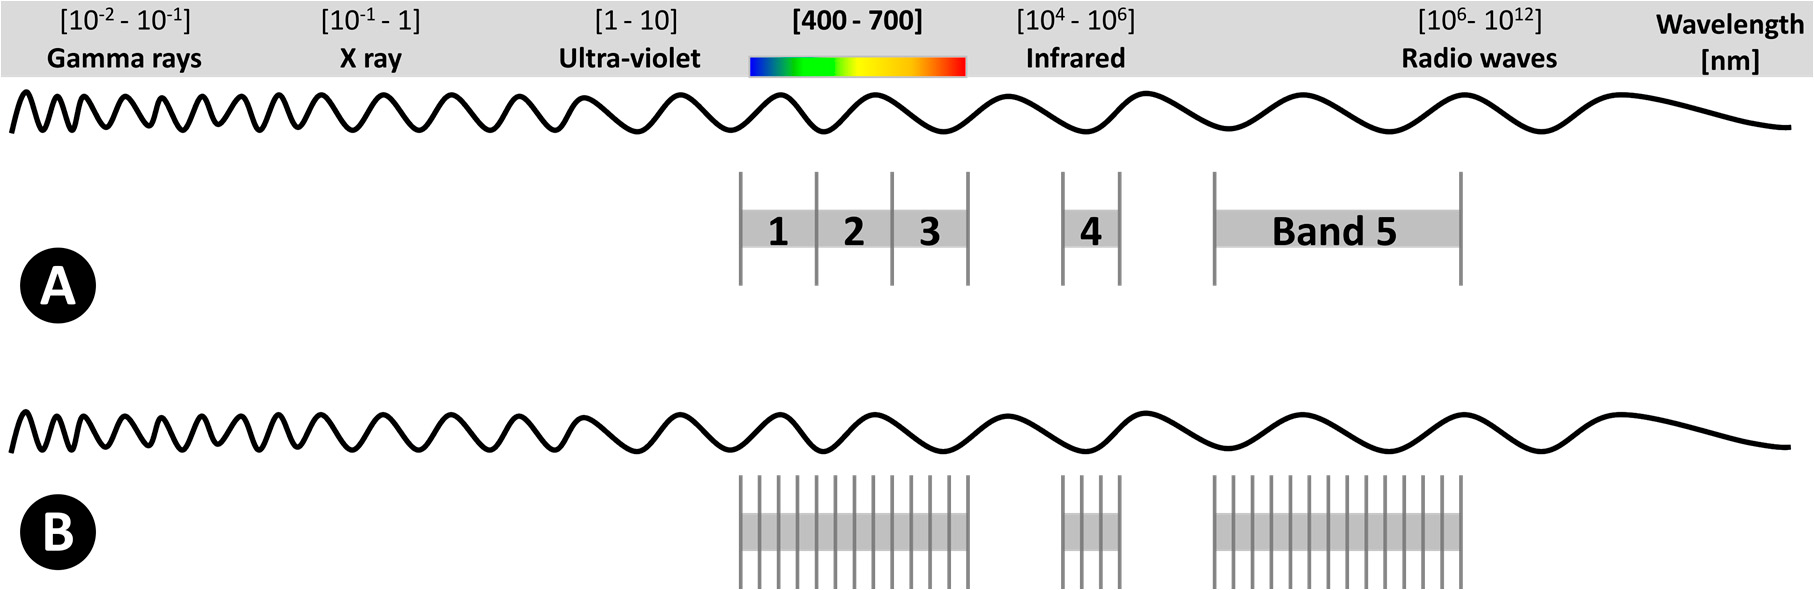
\includegraphics[scale=0.2]{Figs/plan_de_tesis/multivshyper.png}
	\caption{ Representación de los espectros: (A) Multiespectral: 5 
		bandas anchas; y, (B) Hiperespectral: muchas bandas muy estrechas, 
		generalmente entre cientos y miles de ellas. Los dibujos no se 
		encuentran 
		realizados a escala. Imagen tomada de \cite{Adao2017}.}
	\label{fig:spectrus}
\end{figure}


Las cámaras de adquisición de imágenes hiperespectrales estándard utilizan 
redes de difracción o prismas como elementos dispersivos de la luz. La 
distancia requerida entre el sensor de detección y  el componente de difracción 
de la luz, hace que este tipo de cámaras sean muy grandes y muy pesadas, dos 
condiciones que por ejemplo en la industria satelital se quieren optimizar 
fuertemente ya que el costo de la puesta en órbita de los satélites es 
proporcional a su peso y a su tamaño. Estas cámaras suelen ser muy caras y muy 
sensibles a desalinearse debido a las condiciones mecánicas de su construcción. 
Esta última condición se agrava en sistemas de difícil manipulación como lo son 
los satélites, que una vez que se encuentra en órbita, sus componentes ópticos 
ya no puede ser modificados como para corregir una desalineación que empeore la 
calidad de las imágenes capturadas. Además, requieren de una rendija 
para poder obtener una alta resolución espectral, lo que restringe 
significativamente la intensidad de la luz a detectar.

En respuesta a las desventajas de las cámaras estándard de imágenes 
hiperespectrales, aparecieron otro tipo de cámaras que utilizan filtros de 
interferencia de banda y que resultaron en un producto final robusto, compacto, 
de bajo costo y de muy buen rendimiento. Una cámara de vuelo 
de este tipo fue desarrollada en la tesis de licenciatura de Agustina Pose bajo 
la dirección de Hernán Grecco \cite{Pose2017} como se mencionó anteriormente. 
La cámara desarrollada tiene la gran ventaja de no presentar partes móviles, 
evitando posibles desalineaciones de los componentes ópticos. Las partes 
móviles de la cámara que serían útiles para realizar un barrido espectral de 
una cierta escena a capturar, no son necesarias pues el barrido es realiizado 
por el movimiento propio del satélite respecto de la Tierra. El esquema básico 
de este tipo de 
cámaras hiperespectales se muestra 
en la Figura \ref{fig:camsens}. Los filtros de interferencia de banda 
utilizados en este tipo de cámaras deben cumplir ciertos requisitos de calidad 
(no presentar rayones, ni marcas, etc) 
y ciertas características espectrales y de transmisión antes de ser 
incorporados a la carga útil de, por ejemplo, un satélite que va a ser puesto 
en 
órbita. En consecuencia, resulta fundamental caracterizar completamente dichos 
filtros antes de construir las cámaras de la aplicación de interés.

\begin{figure}[H]
	\centering
	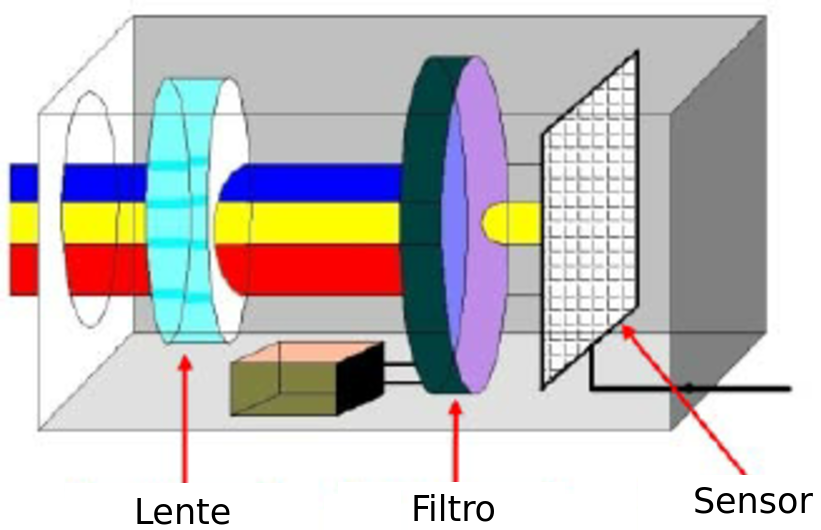
\includegraphics[scale=0.535]{Figs/plan_de_tesis/cam_sens.png}
	\caption{ Esquema de una cámara hiperespectral. El filtro absorbe el 
	espectro completo de la luz incidente salvo la banda espectral que el 
	usuario determina, por lo que sólo las longitudes de onda elegidas 
	atraviesan el filtro y son detectadas por el sensor. \cite{Martinez2008}}
	\label{fig:camsens}
\end{figure}



Debido a las limitaciones de las técnicas de 
medición estándard 
de los espectros de transmisión de los filtros ópticos donde se utilizan 
espectrómetros comerciales, existen tres discrepancias fundamentales 
entre el espectro ''real''\footnote{El espectro ''real'' es 
	el espectro de diseño del filtro para el que fue especialmente construido.} 
	de 
un 
filtro y sus mediciones experimentales realizadas con 
espectrómetros comerciales (Ver Figura \ref{fig:obj1a})\cite{Semrock}. La 
primera discrepancia es el "redondeo" de características espectrales nítidas de 
los filtros. 
Esto se debe al ancho de banda no nulo del haz de la sonda del 
espectrómetro. 


La segunda discrepancia se debe al rango limitado de 
medición de la OD\footnote{La densidad óptica, OD (Optical Density), es un 
	parámetro útil para describir la transmisión de la luz a través de un 
	filtro 
	óptico con una transmisión extremedamente baja. Si T es la transmisión del 
	filtro, que varía entre 0 y 1, se define la densidad óptica como $OD = 
	-$log$_{10} (T)$.} del filtro, que es 
producto de la sensibilidad limitada del espectrómetro. Cuando un filtro 
tiene un valor de OD muy alto, OD $>$ 6, el detector debería medir una 
intensidad de la luz prácticamente nula pero el ruido óptico y electrónico 
propio del detector limita el nivel más bajo de intensidad que puede medir 
con precisión. De esta forma, se puede ver un ruido de piso debido al 
sensor indicando un cierto valor de OD que no coincide con el valor real 
del filtro.

\begin{figure}[H]
	\centering
	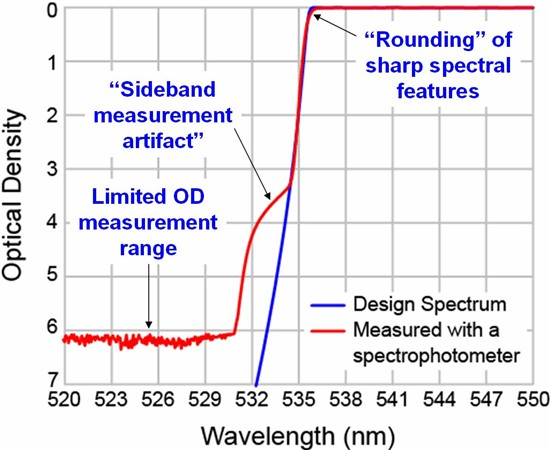
\includegraphics[scale=0.8]{Figs/plan_de_tesis/measurement_of_optical_filter.jpg}
	\caption{Discrepancias entre las mediciones experimentales con 
		espectrómetros 
		comerciales y el espectro ''real'' de un filtro óptico. Adaptado de 
		\cite{Semrock}.}
	\label{fig:obj1a}
\end{figure}

La tercera 
discrepancia es propia de las mediciones de transiciones muy 
pronunciadas. Esto surge 
por el hecho de que el 
haz de la sonda no es monocromático, sino que también tiene bandas 
laterales débiles de longitudes de onda fuera de su ancho de banda 
principal.

Las discrepancias de medición en espectrómetros convencionales 
causan 
importantes problemas al intentar evaluar el rendimiento del filtro para la 
aplicación prevista. 

La elección del instrumento de medición y la técnica 
empleada determinan la precisión de la medición del espectro de transmisión del 
filtro. Al mismo tiempo, determinan la duración y por ende también el costo de 
dichas mediciones, que deben ser compatibles con los tiempos que la industria 
requiere. Esto se puede ver con un ejemplo tomado de \cite{Semrock}. En la 
Figura \ref{fig:may_dists} se muestran cinco mediciones distintas de 
la densidad óptica de un filtro diseñado para bloquear longitudes de onda de 
532 nm con OD $>$ 6 y tener una transición a un estado de alta transmisión 
dentro del $0.5\%$ de la longitud de onda del láser utilizado para excitar la 
muestra, que es de 534.7nm.


\begin{figure}[H]
	\centering
	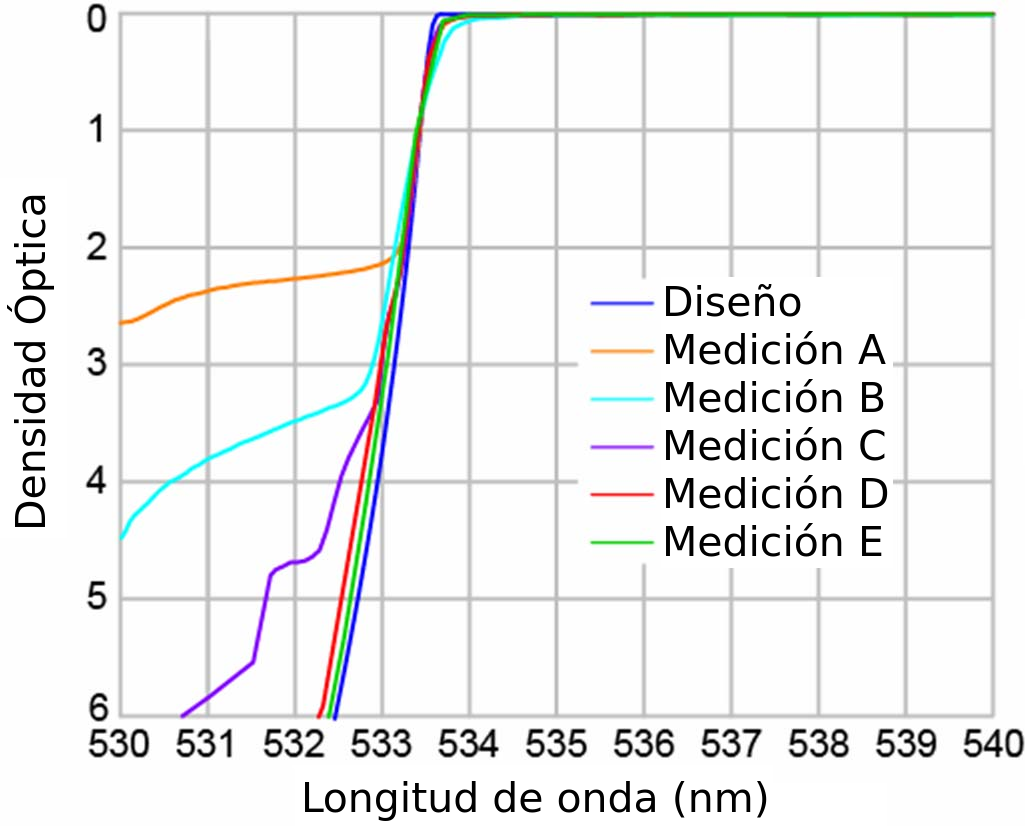
\includegraphics[scale=0.8]{Figs/plan_de_tesis/dists_meds.png}
	\caption{Distintas mediciones de la OD de un filtro LP03-532RE-
		25 RazorEdge de la empresa Semrock. Las mediciones fueron realizadas 
		utilizando tanto espectrómetros comerciales como \textit{custom-made} 
		de la emppresa con una variedad de arreglos experimentales que se 
		explican en el texto. Adaptado de 
		\cite{Semrock}.}
	\label{fig:may_dists}
\end{figure}

Las mediciones del método A fueron realizadas por un espectrómetro de diseño 
propio (\textit{custom-built}) de la empresa,  que tiene un tiempo de 
integración muy corto y una baja resolución, lo que resulta en una 
configuración 
experimental óptima para obtener mediciones de una gran cantidad de filtros de 
prueba. Este método es utilizado para determinar con precisión la longitud de 
onda a partir de la cual el filtro pasa a tener una alta transmisión, es decir, 
localiza la longitud de onda de la transición entre el estado de bloqueo y de 
transmisión del filtro, la longitud de onda de corte. De esta forma, se 
garantiza una cierta uniformidad en un lote de filtros a ser utilizado de una 
forma rápida y eficiente. Ahora bien, como se observa en el gráfico de la 
Figura \ref{fig:may_dists}, el método A posee una sensibilidad muy mala y una 
resolución muy baja, obteniéndose un piso de ruido mayor a OD 2.

El método B utiliza un espectrómetro comercial (Perkin Elmer
Lambda 900) cuyos inconvenientes fueron explicados a partir de las tres 
discrepancias en la Figura \ref{fig:obj1a}. Con este método no se puede 
asegurar que el filtro tenga un 0D $>$ 6 en los 532nm.


Los métodos C y D utilizan el mismo espectrómetro \textit{custom-built}	del 
método A, cuyo principio de funcionamiento básico se muestra en la Figura 
\ref{fig:med_prev}. La diferencia fundamental con el método B que utiliza un 
espectrómetro comercial es que las mediciones con el espectrómetro 
\textit{custom-built} realizan la detección con una cámara CMOS de bajo ruido, 
que consiste en un arreglo de detectores, por lo que puede medir en un rango 
muy grande de longitudes de onda simultáneamente. Este método permite en 
consecuencia obtener mediciones en un rango espectral muy grande, con una 
cierta resolución en un cierto tiempo de integración, de forma muy rápida.
El inconveniente fundamental de este método es que al utilizar una fuente de 
iluminación de banda ancha, si el filtro de prueba tuviera, por ejemplo, una 
autofluorescencia apreciable \cite{Shah2017}, podría interferir con una 
medición precisa de la transmisión de la muestra.


\begin{figure}[H]
	\centering
	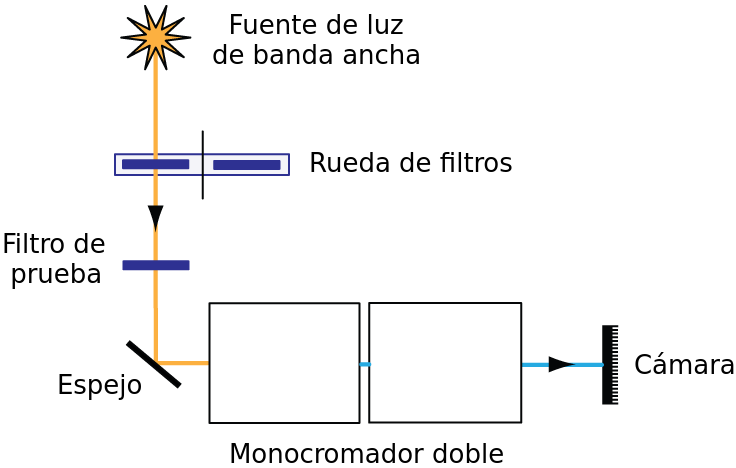
\includegraphics[scale=0.8]{Figs/plan_de_tesis/med_mets_prevs.png}
	\caption{Diseño básico de un espectrómetro \textit{custom-built} que 
	utiliza una fuente de iluminación de banda ancha y permite la recolección 
	de una 		amplia gama de
		longitudes de onda simultáneamente con un conjunto de detectores 
		situados en la cámara. Este 
		arreglo experimental permite una medición más rápida con un piso de 
		ruido y una resolución fijas. Adaptado de 
		\cite{Semrock}.}
	\label{fig:med_prev}
\end{figure}




Ahora bien, dependiendo de la aplicación, las limitaciones en las mediciones 
del espectro de transmisión de los filtros pueden ser determinantes o no. En el 
presente proyecto se quiere determinar el arreglo experimental óptimo pero que 
sea compatible con los tiempos y costos de producción de la industria satelital.

En ciertos filtros y aplicaciones, resulta de vital importancia 
el 
nivel de bloqueo de ciertos rangos de longitudes de onda pero no así la 
suavidad de la transición entre el bloqueo y la transmisión. Por ejemplo, en 
sistemas de 
imágenes de fluorescencia los espectros de absorción y emisión del fluróforo 
podrían estar lo suficientemente alejados como para que resulte fundamental que 
los filtros de banda de la señal de respuesta (de emisión) de la muestra tengan 
un bloqueo muy alto en la banda de la señal de excitación y así lograr una 
relación entre la señal y el ruido de adecuada proporción \cite{Grecco2016}. 

Los filtros 
diseñados para estas aplicaciones podrían tener decenas de OD de bloqueo pero 
en 
la práctica incluso el más pequeño de los defectos físicos en los 
recubrimientos ópticos (\textit{coatings}) o en el montaje, así como el bajo 
nivel de control de luz parásita a nivel del sistema, puede limitar el 
bloqueo alcanzable a valores mucho menores que los del diseño original, en el 
rango de aproximadamente OD 6 a quizás 10.%(forma indirecta de medir los scrath 
%and dig!!**))) 

Dado que los espectrómetros 
comerciales estándard tienen una medición de OD de rango limitado debido al 
ruido de fondo del instrumento, se propone un arreglo experimental inicial para 
poder medir los niveles de bloqueo más altos con precisión como se muestra en 
la Figura \ref{fig:su} y que resulta compatible con la producción industrial 
deseada por su simplicidad.


\begin{figure}[h!]
	\centering
	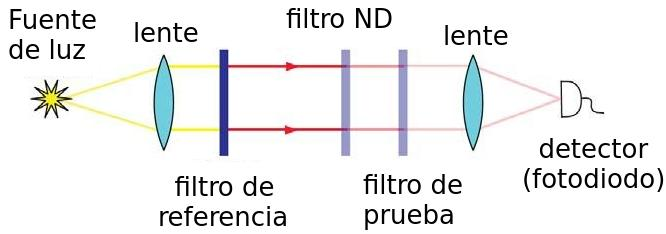
\includegraphics[scale=1.0]{Figs/plan_de_tesis/setup_u.jpeg}
	\caption{Arreglo experimental compatible con la producción industrial para 
	medir valores de 
	OD altos.}
	\label{fig:su}
\end{figure}

El método experimental de la Figura \ref{fig:su} se denomina 
\textit{complementary filter method}. Un haz de 
luz de banda ancha, de una lámpara QTH 
(\textit{Quartz-Tungsten Halogen}) ó de arco, aproximadamente colimado por una 
lente  es filtrado utilizando un filtro 
de referencia ampliamente bloqueador, que es esencialmente un filtro de banda 
con su banda de paso superpuesta a la región del espectro del filtro de prueba 
que se quiere analizar donde la medición de valores de OD altos son necesarios. 
La luz transmitida es enfocada con una lente convergente en un detector de bajo 
ruido capaz de medir niveles de intensidad de luz muy pequeños, como un 
fotodiodo de gran área con un circuito amplificador de bajo ruido ó un tubo 
fotomultiplicador (PMT).


Las mediciones se realizan de la siguiente manera. En primer lugar, se mide la 
intensidad de la señal en el detector con solo el filtro de referencia y un 
filtro calibrado de densidad neutra (ND) en la trayectoria de la luz. El filtro 
ND sirve para reducir el nivel de la intensidad de la luz en el detector en 
una cantidad calibrada de forma tal que el bias \footnote{El bias del 
detector es el valor medido por el instrumento cuando no hay ninguna fuente 
de luz incidiendo sobre él, es el valor de \textit{offset} que se le suma a 
cualquier 
medición.} del rango 
dinámico limitado alcanzable por el detector sea reducido para alcanzar los 
niveles de la señal que el detector va a ver cuando se coloquen los filtros de 
prueba. En particular, con un filtro ND 3, el rango dinámico del detector tiene 
que ser de $10^{6}$ para medir hasta un valor de OD 9 de bloqueo. En segundo 
lugar, se retira el filtro ND y se lo reemplaza por el filtro de prueba para 
realizar una nueva medición de la intensidad con el detector. El cociente entre 
las dos mediciones de intensidad de la luz es igual al valor de OD del filtro 
de prueba, en el rango espectral del filtro de referencia.


\section*{Actividades y Metodología}

\hspace{0.5cm}En el presente trabajo de tesis se desarrollarán múltiples 
arreglos 
experimentales para caracterizar el espectro de transmisión de distintos 
filtros de prueba que dispone el LEC, utilizando técnicas de medición en línea 
con los papers y patentes de la actualidad. Se automatizará la adquisición de 
las mediciones y se incorporará al arreglo experimental inicial un sistema de 
detección de defectos de los filtros, utilizando una cámara de bajo costo del 
laboratorio para realizar las primeras pruebas. 

Una vez caracterizado tanto el espectro como los defectos de los filtros, se 
diseñará y construirá un primer prototipo de un sistema integral de 
caracterización para ser aplicado con los filtros que utiliza la empresa 
Satellogic en sus cámaras hiperespectrales. Se estudiará la aplicabilidad de 
este prototipo en distintos casos.

Utilizando el prototipo del sistema integral de caracterización de los filtros 
se desarrollará un método y criterios para decidir si un filtro puede ser 
incorporado a la cámara utilizada en los satélites.

Como aplicación de este proyecto de tesis se utilizarán las cámaras 
hiperespectrales de la empresa Satellogic, cuyos filtros van a ser 
caracterizados con el sistema integral que se va a desarrollar, y se tomarán 
imágenes en tierra utilizando algoritmos de HDR y de búsqueda de 
características.  Y, finalmente se realizará una caracterización de los filtros 
en su posición final en las cámaras de vuelo del satélite.

El cronograma mensual de trabajo se muestra en la siguiente Tabla:

%\begin{tcolorbox}[tab2,tabularx={X||Y|Y|Y|Y|Y|Y|Y|Y|Y|Y|Y|Y},title= 
%\textbf{Cronograma mensual de actividades propuestas},boxrule=0.5pt]
%	\textbf{Actividad} & \textbf{4} & \textbf{5} & \textbf{6} & 
%	\textbf{7} & \textbf{8} & \textbf{9} & \textbf{10} & \textbf{11} & 
%	\textbf{12}      
%	\\\tcbline\tcbline
%	Revisión del estado del arte   &  \checkmark    &  & & & & & & & \\\tcbline
%	Caracterización de los espectros de transmisión de los filtros    &   & 
%	\checkmark & \checkmark
%	& \checkmark & & & & &\\ \tcbline
%	Determinación de defectos de los filtros (\textit{scratch and dig})     &   
%	&  & \checkmark & \checkmark & & & & &\\ \tcbline
%	Diseño y construcción del primer prototipo del sistema integral de 
%	caracterización de los filtros    &   
%	&  &  & \checkmark & \checkmark & & & &\\ \tcbline
%	Implementación del sistema integral en las cámaras de Satellogic. 
%	    &   
%	&  &  &  & \checkmark & \checkmark & \checkmark & &\\\tcbline
%	Procesamiento de imágenes haciendo HDR y búsqueda de características  &   
%	&  &  &  & \checkmark & \checkmark & \checkmark & \checkmark &\\\tcbline
%	Caracterización de los filtros en su posición final en las cámaras de vuelo 
%	del satélite   &   
%	&  &  &  & &  &  & \checkmark & \checkmark \\\tcbline
%\end{tcolorbox}



\section*{Factibilidad}

\hspace{0.5cm}El lugar de trabajo donde el tesista va a desarrollar sus 
actividades es el 
Laboratorio de Electrónica Cuántica (LEC) del Departamento de Física de la 
Facultad de Ciencias Exactas y Naturales, UBA. El LEC cuenta con diversos 
equipos de uso general en óptica y electrónica y algunos de uso específico para 
aplicaciones en investigación de física básica. Entre los equipos de uso 
relevante para el presente proyecto se pueden encontrar mesas ópticas de 
suspensión neumática, un microscopio invertido automático Zeiss Observer Z1, 
diversas placas de adquisición y procesamiento (NI y Red Pitaya, Raspberry Pi y 
Arduino), cámaras científicas y de bajo ruido (Apogee U2000, QHY183M), 
elementos de óptica para la construcción de instrumentos (lentes, filtros, 
objetivos de microscopio, optomecánica, láseres y leds). Adicionalmente, el 
laboratorio cuenta con acceso a un microscopio confocal de la firma Olympus, 
modelo FV1000 equipado con una platina motorizada, cámara ambiental y cámara 
CCD.
 
El director de la presente tesis es director del LEC y es experto en temas de 
óptica y fotofísica, áreas principales del proyecto. Además, tiene la 
experiencia de haber dirigido a una estudiante que realizó la tesis en conjunto 
con el LEC y la empresa Satellogic, resultando en una experiencia exitosa.

El tesista se encuentra cursando actualmente sus últimas dos materias de la 
carrera: 
Estructura de la Materia 4 e Instrumentación y Control.





\chapter{Primer prototipo del equipo y caracterización de los espectros de transmisión}

%%%%%%%%%%%%%%%%%%%%%%%%%%%%%%%%%%%%%%%%%%%%%%%%%%%%%%%%%%CAPITULO 3:%%%%%%%%%%%%%%%%%%%%%%%% Cuantificación de los defectos a partir de las imágenes tomadas con el ZEISS con scikit-image y OpenCV %%%%%%%%%%%%%%%%%%%%%%%%%%%%%%%%%%%%%%
%%%%%%%%%%%%%%%%%%%%%%%%%%%%%%%%%%%%%%%%%%%%%%%


%\Chapter{Cuantificación de los defectos a partir de las imágenes tomadas con el ZEISS con scikit-image y OpenCV}{\textcolor{MidnightBlue}{\faGithub \href{https://github.com/jrr1984/defects_analysis}{\texttt{defects$\_$analysis}}}}

\singlespacing
\Chapter{Cuantificación de los defectos}{\textcolor{MidnightBlue}{\faGithub \href{https://github.com/jrr1984/defects_analysis}{\texttt{defects$\_$analysis}}}}
\spacing{1.5}

\hspace{0.5cm}En este capítulo se define qué es lo que se considera un defecto de un componente óptico, se muestran las características del filtro óptico utilizado en el presente trabajo y la cuantificación de los defectos de cada una de las bandas espectrales que el filtro presenta. Se explica el proceso de adquisición de las imágenes de cada banda del filtro y su posterior procesamiento. 

Asimismo, se detalla el algoritmo utilizado para realizar la detección de los defectos en las imágenes adquiridas y se analizan los resultados: número de defectos por unidad de superficie, diámetro y área de los defectos, etc. Finalmente, considerando las reglamentaciones vigentes en la industria, se explica la aplicación de criterios de normas de calidad que permiten determinar que el filtro analizado \underline{no} cumple las especificaciones técnicas necesarias para ser montado en un sensor de imagen para aplicaciones aeroespaciales.

\singlespacing
\section*{Defectos de superficie de un componente óptico}
\label{sec:defectsurf}
\spacing{1.5}

\vspace{1.0cm}
\todo[inline]{Cómo asociar errores a las dimensiones medidas tanto con el fiji como con el algoritmo. Al error de las imágenes del zeiss se le pone la calibración, por ej $\pm$ 0.586 $\mu$m , aprox 0.59 micrones de error }
\vspace{1.0cm}

\hspace{0.5cm}Se define un defecto de superficie de un componente óptico de manera general como una imperfección localizada, es decir una ruptura de la homogeneidad de la superficie óptica \cite{Gomez_1998}. Estas imperfecciones consisten de rayones (en inglés \textit{scratches}), hoyos (en inglés, \textit{digs}), huecos, manchas, burbujas, entre otras consideradas en las especificaciones estándard de la industria. La terminología varía dependiendo del sector de la industria óptica que se trate. En particular, en el presente trabajo se caracterizaron defectos de superficie denominados en adelante huecos (Ver Figura \ref{fig:huecocel}) y manchas ó defectos de transmisión (Ver Figura \ref{fig:manchacel}). 

\begin{figure}[H]
	\begin{floatrow}
		\ffigbox{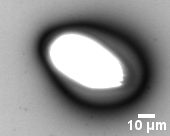
\includegraphics[width=4.0cm,height=4.0cm]{Figs/cuantificaciondefectos/hueco_cel_112.png}}{\caption{Defecto de superficie denominado hueco, de (48.45 $\pm$0.59)$\mu$m de diámetro equivalente. }\label{fig:huecocel}}
		\ffigbox{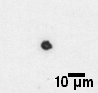
\includegraphics[width=4.0cm,height=4.0cm]{Figs/cuantificaciondefectos/mancha_cel_112.png}}{\caption{Defecto de superficie denominado mancha ó defecto de transmisión, de (6.33 $\pm$0.59)$\mu$m de diámetro equivalente.}\label{fig:manchacel}}
	\end{floatrow}
\end{figure}

Los defectos de superficie de un componente óptico pueden estar originados en el proceso de fabricación mismo, en el tratamiento y manipulación de la óptica (en inglés, \textit{handling}) en distintas etapas de un proceso de montaje ó en el transporte del proveedor al cliente. Estos defectos pueden provocar un cambio de las propiedades ópticas del componente, como por ejemplo una merma en la intensidad esperada ó una variación del espectro de tranmisión, y en consecuencia los usuarios finales de los componentes deben verificar la calidad óptica que los proveedores detallan en las especificaciones técnicas. A continuación se describen las dos especificaciones técnicas más utilizadas en la industria para determinar la calidad óptica de un componente, que son la \textit{U.S. Military Performance Specification} MIL-PRF-13830B y la ISO 10110 \cite{milprf}\cite{iso10110}.

\singlespacing
\subsection*{MIL-PRF-13830B: especificaciones de \textit{scratch \& dig}}
\spacing{1.5}

\hspace{0.5cm}La especificación técnica MIL-PRF-13830B define los defectos permitidos en una superficie óptica utilizando una métrica dada por un par de números denominados \textit{scratch and dig numbers}: S/D. El \textit{scratch number} puede tomar alguno de los siguientes valores arbitrarios: 10,20,40,60,80, que representan en orden creciente el nivel de brillo de la rayadura. Este número no proviene de una medición experimental exacta, sino que es el resultado de comparar el brillo de la rayadura del componente a analizar con muestras de rayaduras calibradas como las que se muestran esquemáticamente en la Figura \ref{fig:scratchanddig}, bajo ciertas condiciones de iluminación específicas. En consecuencia, la asignación de un cierto \textit{scratch number} a un componente es una inspección visual subjetiva, es decir que varía de inspector a inspector.


\begin{figure}[H]
	\centering
	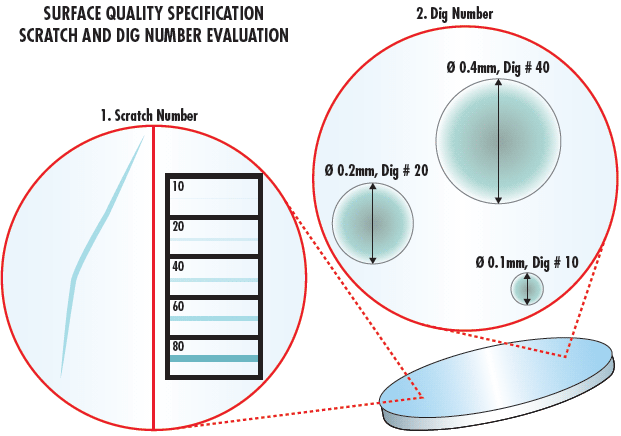
\includegraphics[scale=1.0]{Figs/cuantificaciondefectos/scratchanddig.png}
	\caption{El \textit{scratch number} es determinado a partir de la comparación de la rayadura de la óptica bajo análisis con las muestras calibradas, bajo ciertas condiciones de iluminación específicas. Adaptado de \href{https://bit.ly/2w1apWq}{\texttt{https://bit.ly/2w1apWq}}.}
	\label{fig:scratchanddig}
\end{figure}

Ahora bien, el \textit{dig number} es una cantidad medible experimentalmente: es el diámetro del hoyo más grande del componente, dado en $1/100$ de milímetros. Por ejemplo, un componente con un \textit{dig number} de 40 implica que el hoyo más grande de la óptica tiene un diámetro de 0.4 mm (Ver Figura \ref{fig:scratchanddig}). Luego de cuantificar todas las rayaduras y hoyos de la óptica, se determina el número de defectos permitidos de acuerdo a los siguientes criterios:
\begin{itemize}
\item La suma de todas las longitudes de las rayaduras con un cierto \textit{scratch number} (L$_{S_{\#}}$) no podrá superar el valor de un cuarto del diámetro ($\Phi$) de la óptica. Si el componente no tuviera una geometría circular, se considera el diámetro de un círculo con un área igual al de la óptica bajo análisis.
\begin{equation}
\sum L_{S_{\#}} < \frac{\Phi}{4}
\label{eq:snumb}
\end{equation}
\item El número total de hoyos de tamaño máximo permitido (N) no podrá exceder el diámetro de la óptica dividido por 20.
\begin{equation}
N  <  \frac{\Phi}{20}
\label{eq:nphi20}
\end{equation}
\item La suma de todos los diámetros (d) de los hoyos deberá ser menor ó igual al doble del número total de hoyos de tamaño máximo permitido (N) multiplicado por el \textit{dig number} (D$_{\#}$) especificado en fracciones de milímetros.
\begin{equation}
\sum d 	\leq 2 . N . D_{\#}
\label{eq:dmenorig}
\end{equation}
\end{itemize}


Una óptica de geometría circular con un diámetro de 200 mm y una calidad óptica especificada por el fabricante con \textit{scratch and dig numbers} S/D 20-10, puede tener rayones con un brillo calibrado de 20 y la suma de todas las longitudes de los rayones de brillo 20 no podrá ser superior a los 50 mm (de acuerdo a \eqref{eq:snumb}). Al mismo tiempo, la óptica no podrá tener más de 10 hoyos de tamaño máximo de 0.1 mm, es decir de \textit{dig number} igual a 10 (de acuerdo a  \eqref{eq:nphi20}) y la suma de los diámetros de todos los hoyos no podrá ser superior a los 2 mm (de acuerdo a \eqref{eq:dmenorig}.

La Figura \ref{fig:samplescratchs} muestra una comparación de cuatro muestras de calibración de rayaduras, medidas bajo idénticas condiciones de iluminación \cite{Aikens}.
\begin{figure}[H]
	\centering
	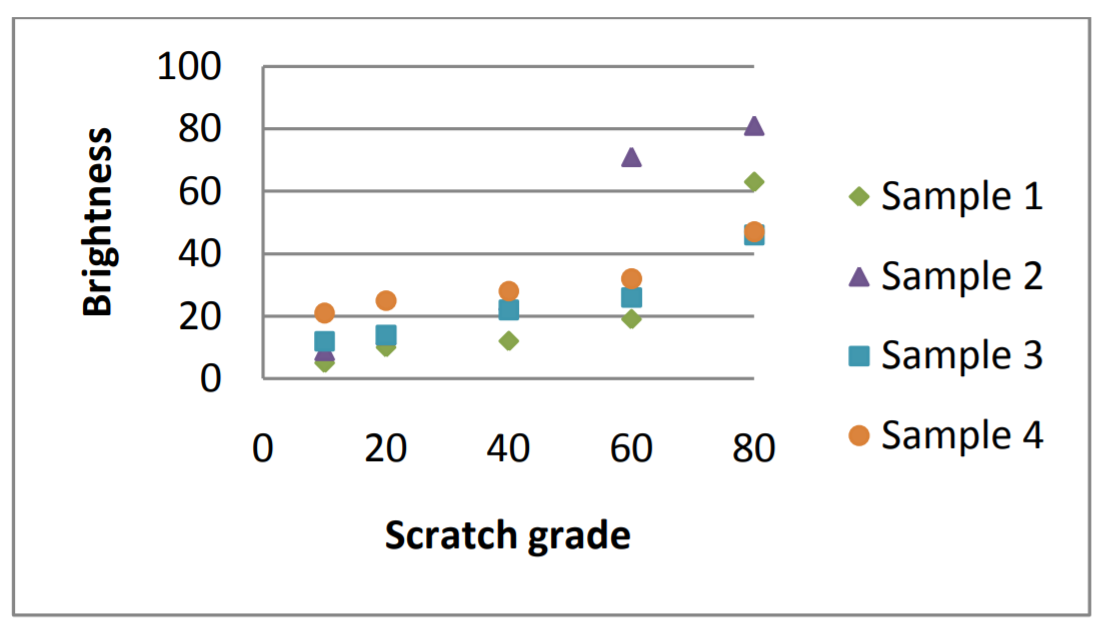
\includegraphics[scale=0.8]{Figs/cuantificaciondefectos/samplesscratch.png}
	\caption{Brillo relativo de cuatro muestras calibradas de \textit{scratch number}. \textit{Sample} en inglés significa muestra. La muestra 1 es de la empresa FLIR/Brysen (S\&D 1109), la muestra 2 es de Davidson Optronics (D-667A S/N 2431), la muestra 3 es de Eastman Kodak Paddle (EKCO CM2) y la muestra 4 es de Jenoptik (\textit{paddle} EO \#53-157 CM1). La muestra 4 es vendida comercialmente por los proveedores Edmund Optics y por Thorlabs. Análisis tomado de \cite{Aikens}.}
	\label{fig:samplescratchs}
\end{figure}


De la Figura \ref{fig:samplescratchs} se desprende que las cuatro muestras son incompatibles entre sí, es decir arrojan resultados de brillo distintos entre sí para un cierto \textit{scratch number}. Se observa que para un \textit{scratch number} igual a 10, el brillo de la muestra 4 es más brillante que el \textit{scratch number} 60 de la muestra 1.
Así también el brillo del \textit{scratch number} 60 de la muestra 2 es más de dos veces más brillante que cualquiera de las otras muestras para este mismo \textit{scratch number}. 

Si bien la métrica de \textit{scratch and dig} sigue siendo ampliamente utilizada en la industria, el hecho de que el análisis de las rayaduras sea dependiente del inspector de turno sumado a que las muestras de brillo calibradas varían de acuerdo al fabricante de las mismas, hacen que estas especificaciones técnicas para determinar la calidad de una óptica resulten técnicamente ambiguas. A continuación se explican las especificaciones técnicas de la ISO 10110 y se hace notar que ambas especificaciones técnicas figuran en la hoja de datos del filtro analizado en el presente trabajo. Luego se muestran las características del filtro analizado en esta tesis junto a sus especificaciones ópticas.

\singlespacing
\subsection*{ISO 10110: defectos de superficie}
\spacing{1.5}


Las especificaciones de la ISO 10110 determinan de forma cuantitativa el tamaño y número de defectos de superficie que un componente óptico puede presentar. El concepto de defecto de superficie para esta normativa se corresponde con la definición de defecto dada en la primera sección de este capítulo (Ver \ref{sec:defectsurf}). Es decir, contiene a todos los tipos de defectos que representan una inhomogeneidad en la superficie óptica del componente. Esto es, no distingue las rayaduras de los hoyos ni de cualquier otro tipo de defecto para determinar la calidad óptica de un componente.

La normativa ISO 10110 indica el número de defectos permitidos ($N_{p}$) y un valor numérico denominado \textit{grade number} ($A_{g}$) que es igual a la raíz cuadrada del área del defecto de tamaño máximo permitido. Estos dos números son expresados en las hojas de datos de los componentes ópticos de la siguiente manera: 5/$N_{p}$x$A_{g}$. El número 5 hace referencia a que la especificación técnica dada se refiere a las tolerancias de los defectos de superficie. Y, el área del componente óptico cubierta por los defectos está dada por la siguiente expresión:

\begin{equation}
A_{defectos} = N_{p} . (A_{g})^{2}
\end{equation}


ISO 10110-7 refers to specifying surface quality through Ng and Ag as the “dimensional” method, but ISO drawings may also indicate surface quality through a “visibility” method identical to MIL-PRF-13830B. 5/60-40 on an ISO print has the same meaning as 60-40 on a print following MIL-PRF-13830B. The benefit of being able to indicate both “dimensional” and “visible” specifications is that it results in prints with all the standardization and lack of notes of an ISO print, with the ability to use the more convenient and cost-effective MIL-PRF-13830B surface quality standard for the majority of applications. The “dimensional” method can then be used for high precision applications where surface quality is of the highest importance.



\singlespacing
\section*{Características del filtro utilizado}
\spacing{1.5}



\singlespacing
\section*{Adquisición de las imágenes del filtro}
\spacing{1.5}


\hspace{0.5cm}Para la adquisición de las imágenes del filtro se utilizó un microscopio invertido Zeiss Axio Observer Z1 como se muestra en la Figura \ref{fig:ZEISSdellabo}, utilizando un objetivo Zeiss N-Achroplan de magnificación 10X y apertura numérica de 0.25.
\begin{figure}[H]
	\centering
	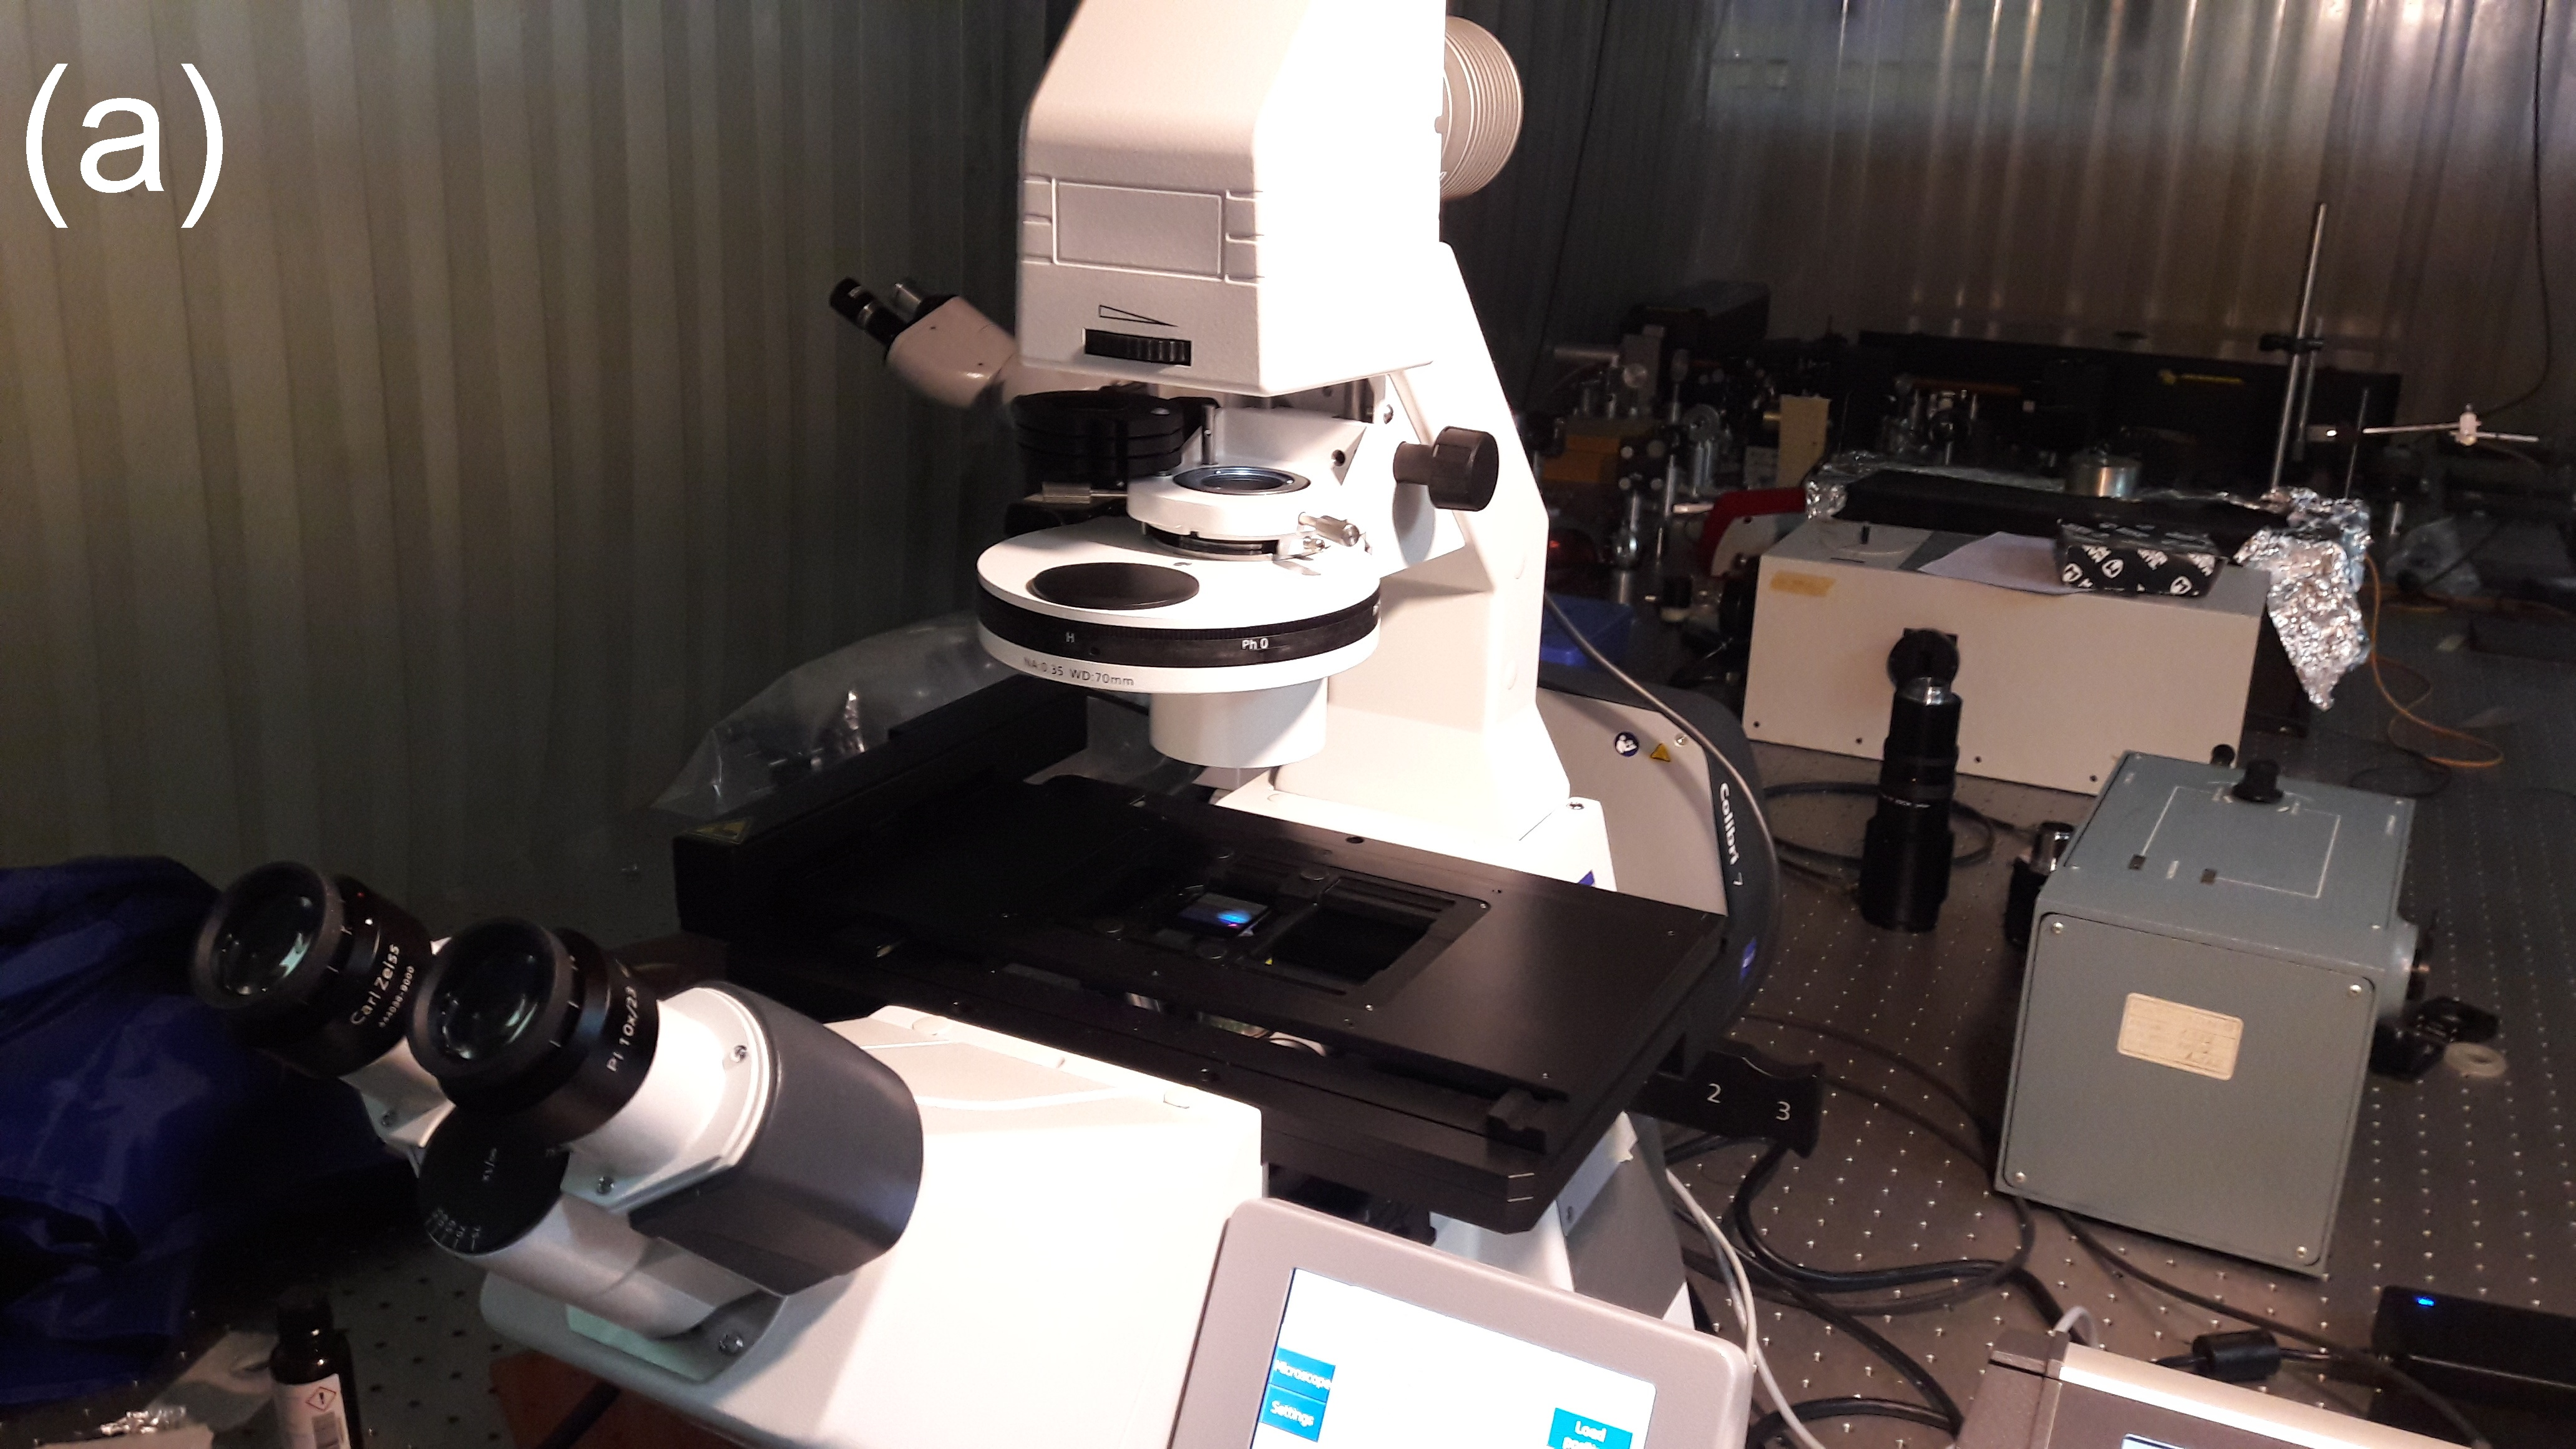
\includegraphics[scale=0.08]{Figs/defectosZEISS/b.jpg}
	\caption{Microscopio invertido Zeiss Axio Observer Z1.}
	\label{fig:ZEISSdellabo}
\end{figure}

Las imágenes del filtro fueron adquiridas por transmisión utilizando una fuente de luz blanca, en condiciones de \textit{bright field}\footnote{Técnica de iluminación que en castellano suele ser denominada de 'campo brillante' para diferenciarla de la iluminación de campo oscuro (en inglés \textit{dark field}).}. Se montó el filtro sobre el portamuestras de la platina del microscopio como se muestra en la Figura \ref{fig:filtroenZEISS} y mirando por el ocular se puso en foco la superficie del filtro a medir.  
\begin{figure}[H]
	\centering
	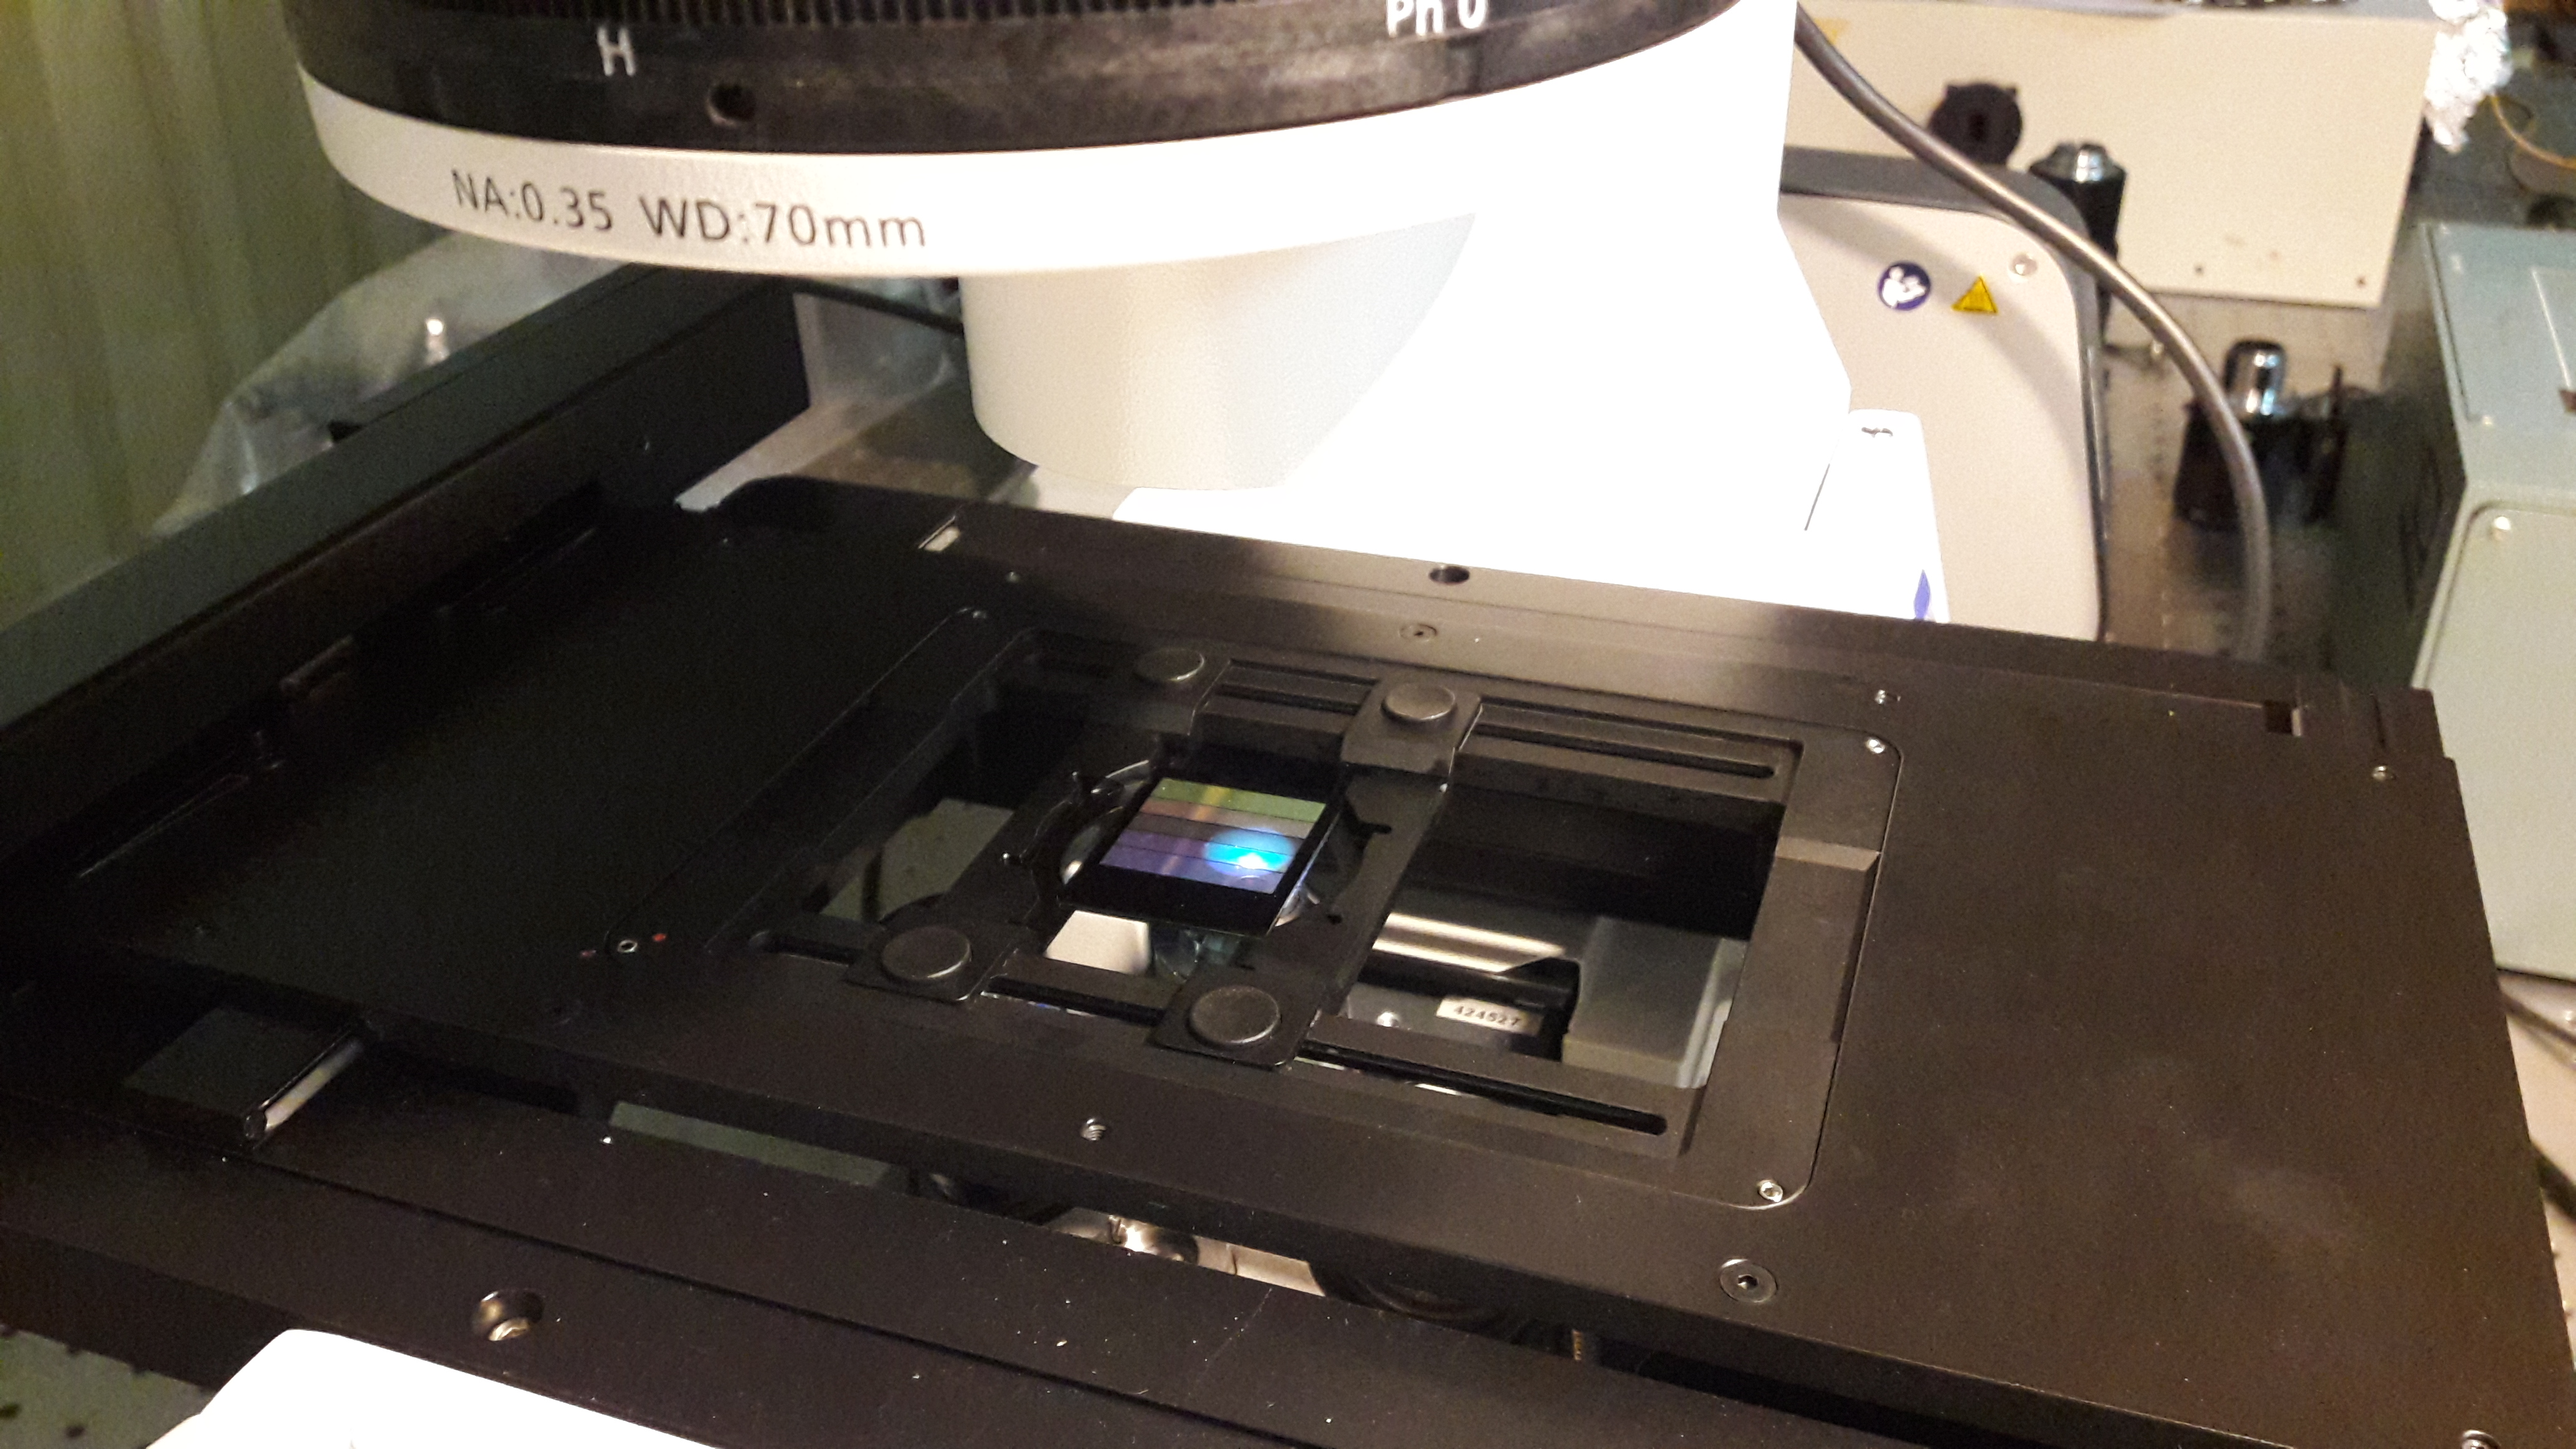
\includegraphics[scale=0.08]{Figs/defectosZEISS/a.jpg}
	\caption{Montaje del filtro sobre el portamuestras de la platina del microscopio.}
	\label{fig:filtroenZEISS}
\end{figure}
La cámara monocromática del microscopio del fabricante Zeiss, modelo Axiocam 702, con un sensor CMOS de 1/1.2'' (diagonal de 13.3mm) y 2.3 megapíxeles, fue controlada a través del software ZEN 2.5 (Blue edition, 2018) del mismo fabricante. Se utilizó la calibración de la cámara que viene de fábrica del microscopio, donde las medidas de 1 pixel son de a 0.586 $\mu m$ x 0.586 $\mu m$.

Se configuró el software para adquirir las imágenes por transmisión, en particular se eligió la fuente de luz blanca y para cada medición su intensidad, además del tiempo de exposición de la cámara. Como la cámara tiene otro arreglo óptico que el ocular, el plano focal de la superficie del filtro elegida para medir se encuentra a una distancia distinta entre el objetivo y la muestra. En consecuencia, con las perillas manuales del microscopio se pone en foco la imagen observando la adquisición en vivo en la computadora.

\vspace{1.0cm}
\todo[inline]{no medi con el ocular entonces no decir nada del ocular.}
\vspace{1.0cm}

\singlespacing
\subsection*{\textit{Tile scan}}
\spacing{1.5}

\hspace{0.5cm}A continuación se explica cómo se adquirieron las imágenes para una determinada región del filtro, ya sea para el filtro completo a excepción de la banda del NIR\footnote{NIR, en inglés \textit{Near-Infrared}, se le denomina a la región espectral del infrarrojo cercano que se extiende aproximadamente desde los 780 nm hasta los 2000 nm.} ó para cada banda espectral del filtro en particular.

La palabra en inglés \textit{tile} significa baldosa(ver Figura \ref{fig:tilescan}) en castellano y realizar un \textit{tile scan} implica realizar un barrido de adquisición de imágenes de una cierta área a elección de una muestra donde el área total a adquirir está compuesta por múltiples baldosas. Cada baldosa, es decir cada \textit{tile} constituye una imagen del microscopio de acuerdo al \textit{field of view} (FOV) \footnote{En castellano es el campo de visión y representa el área física de la imagen, que para el caso de una cámara el FOV viene dado por el cociente entre el tamaño del sensor CMOS y la magnificación del microscopio.} que se tiene del arreglo óptico de la cámara integrada al microscopio.

Hay distintas formas de elegir el área total a adquirir en el software. Se eligió la opción de determinar la región a adquirir a partir de la selección visual individual de las cuatro esquinas de la misma, como se muestra en la Figura \ref{fig:tilescan}. Para elegir estas esquinas el microscopio cuenta con un \textit{joystick} que permite mover la platina motorizada del microscopio en el plano de la imagen.

\begin{figure}[!h]
	\centering
	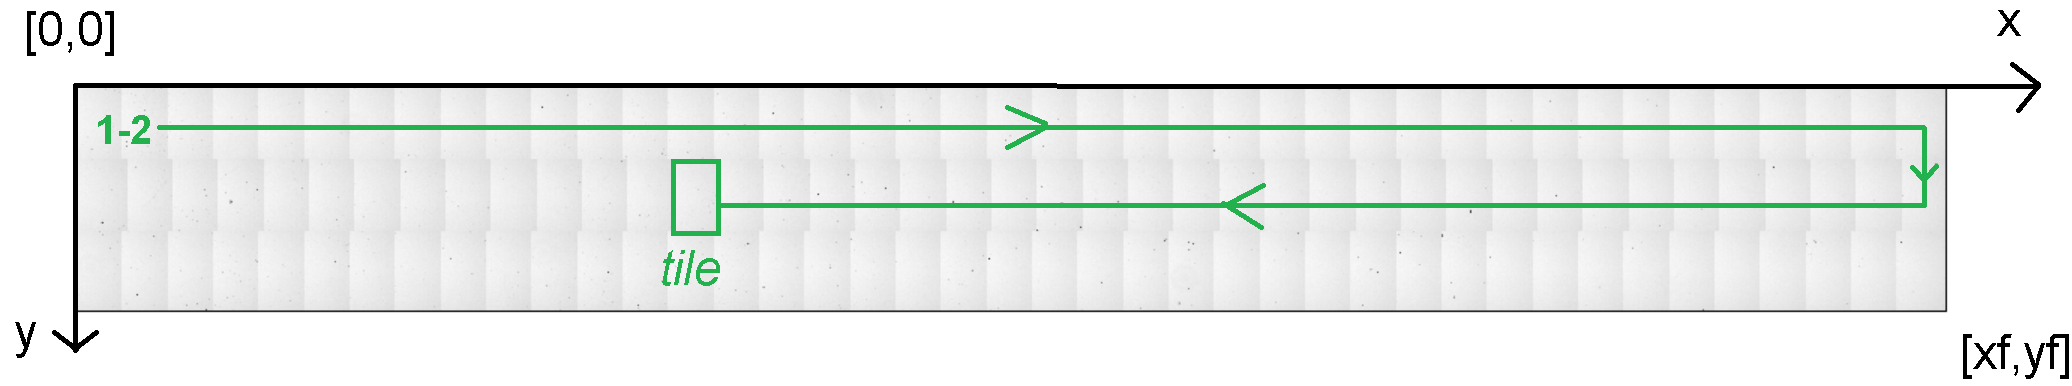
\includegraphics[width=1.0\textwidth]{Figs/cuantificaciondefectos/tilescan.png}
	\caption{\textit{Tile scan} de la banda pancromática.}
	\label{fig:tilescan}
\end{figure} 

Entre otros parámetros del barrido, se elige el \textit{overlap} entre las baldosas, es decir la superposición entre las mismas que luego permite obtener una imagen completa individual,  realizando un \textit{stitching}\todo{explicar que es lo que hace el software}\footnote{El \textit{stitching} de las imágenes (baldosas) es el 'pegado' de cada una con sus vecinas para que en la imagen final no se observen los bordes de cada baldosa sino que la imagen completa se vea como si hubiese sido adquirida individualmente.} como post-procesamiento de las imágenes. Este último procedimiento también fue realizado con el software de Zeiss. Se configuró el \textit{overlap} en 10$\%$ para todas las mediciones\todo{explicar mas xq el 10 porciento con ayuda del stitching}, siendo este valor el mínimo encontrado para que el \textit{stitching} entre las imágenes consecutivas sea realizado correctamente sin dejar espacios en blanco y para que dicha superposición elimine de la imagen la menor cantidad de defectos posibles. Por último, se elige en la configuración que cada baldosa sea exportada como una imagen individual para su posterior análisis.

\singlespacing
\subsection*{Superficies y mapa de los defectos del filtro}
\spacing{1.5}

\vspace{1.0cm}
\todo[inline]{presentar el filtro real, con las dimensiones}
\vspace{1.0cm}

\hspace{0.5cm}Se adquirieron imágenes completas del filtro, a excepción de la banda espectral del NIR, para las dos superficies exteriores del filtro como se muestra en las Figuras \ref{fig:supfiltrocondensador} y \ref{fig:supfiltroobjetivo}.

\begin{figure}[H]
	\begin{floatrow}
		\ffigbox{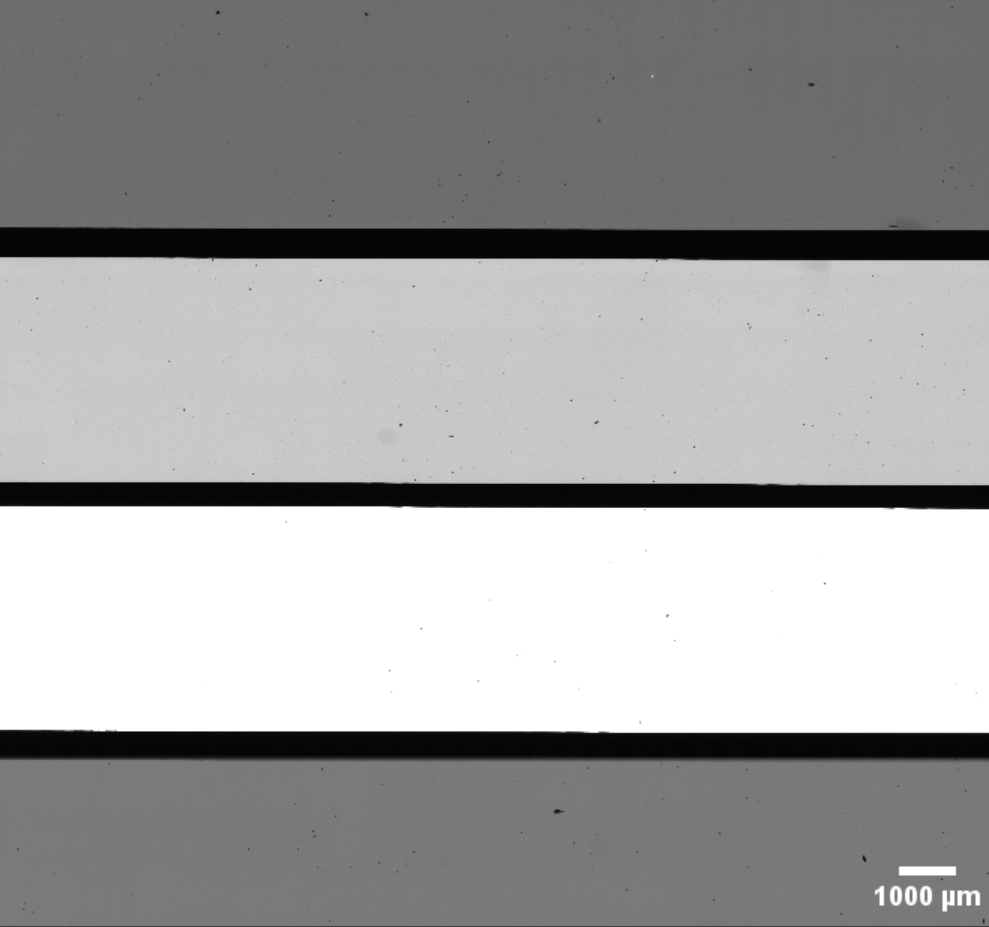
\includegraphics[width=7.25cm,height=9.0cm]{Figs/cuantificaciondefectos/supfiltrocondensador.png}}{\caption{Imagen de la superficie exterior superior del filtro, para un barrido de 15.18 mm x 15.30 m.}\label{fig:supfiltrocondensador}}
		\ffigbox{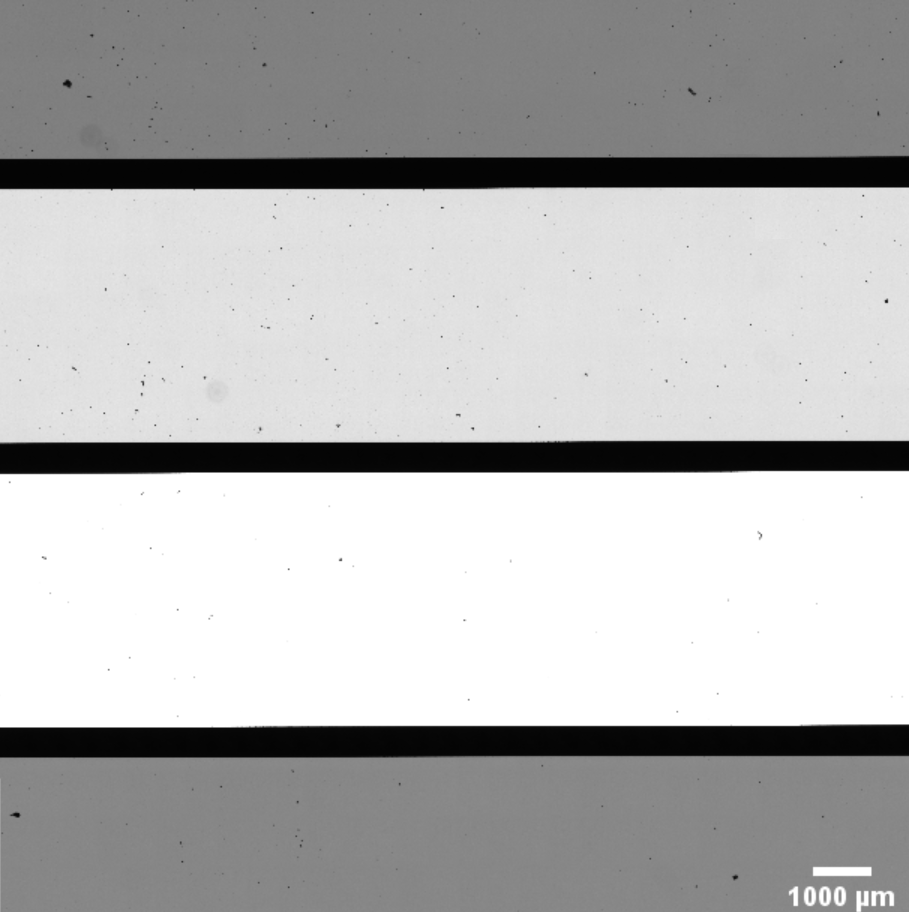
\includegraphics[width=7.25cm,height=9.0cm]{Figs/cuantificaciondefectos/supfiltroobjetivo.png}}{\caption{Imagen de la superficie exterior inferior del filtro, para un barrido de 22.09 mm x 16.24 mm.}\label{fig:supfiltroobjetivo}}
	\end{floatrow}
\end{figure}

\vspace{1.0cm}
\todo[inline]{imagenes de las mismas dimensiones, recortarlas lo que sea. Escala verde y roja por ejemplo}
\vspace{1.0cm}


En las Figuras \ref{fig:supfiltrocondensador} y \ref{fig:supfiltroobjetivo} se muestran las bandas espectrales del filtro en orden descendente: Celeste (450-510 nm), Verde (510-580 nm), Pancromática (450-750 nm), Roja (590-690 nm). El brillo, el contraste y el tamaño de las imágenes originales fueron modificados para obtener una mejor visualización, utilizando el software FIJI-ImageJ. 

\vspace{1.0cm}
\todo[inline]{ponerlo en la presentacion oficial del sr filtro}
\vspace{1.0cm}

Para realizar el barrido completo de cada superficie se verificó en las cuatro esquinas de la superficie a medir que no se pierda el foco de la imagen. Se eligió la intensidad de la fuente de luz y el tiempo de integración de la cámara tales que no saturen alguna de las bandas del filtro de forma tal poder adquirir una imagen completa del filtro en un solo barrido, y de forma tal que se utilice la mayor parte del rango dinámico de la cámara, como se muestra en la Figura \ref{fig:histograma15x15} el histograma de la intensidad de los píxeles de la cámara para el barrido de la Figura \ref{fig:supfiltrocondensador}.

\begin{figure}[!h]
	\centering
	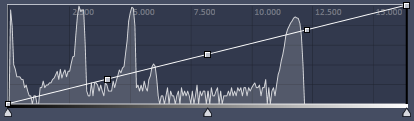
\includegraphics[width=1.0\textwidth]{Figs/defectosZEISS/histograma15x15.png}
	\caption{Histograma de la intensidad de los píxeles de la cámara del barrido de la superficie exterior superior del filtro.}
	\label{fig:histograma15x15}
\end{figure}
 
\vspace{1.0cm}
\todo[inline]{oracion de abajo es super larga, reescribir y partir en 2 por lo menos}
\vspace{1.0cm}

Se hace notar que la banda del NIR no pudo ser adquirida en el barrido completo de las superficies exteriores del filtro pues con los valores de intensidad de la lámpara y del tiempo de adquisición de la cámara fijados para que ninguna de las bandas del filtro sature\todo{quedo muy informal, ponerlo en infinitivo Aumentar estos dos paSi se aumentaban estos dos parámetros de la adquisición se saturaba en particular la banda espectral pancromática.}, no era posible obtener una buena calidad de la imagen en esa banda. Si bien la cámara tiene un rango de sensibilidad espectral comprendido entre los 350 nm y los 1000 nm de acuerdo a su hoja de datos \cite{Zeiss}, del gráfico de la eficiencia cuántica\footnote{La eficiencia cuántica, en inglés \textit{Quantum efficiency} (QE), es una medida precisa de la sensibilidad de un dispositivo fotosensible que permite determinar como es la respuesta del dispositivo para cada longitud de onda.} se desprende que para la región espectral del NIR tiene una eficiencia cuántica menor al 30\% (Ver Figura \ref{fig:eficienciacuanticamara}). A esto se le suma el hecho de que la fuente de luz tiene un espectro de emisión de baja intensidad en la región del NIR, como se muestra en la Figura \ref{fig:espectrolamparazeiss}. Dicho espectro fue medido con el espectrómetro CCS200 de Thorlabs. Ahora bien, la banda espectral del NIR fue medida individualmente posteriormente como se explica más adelante.
Para poder obtener una imagen del filtro completo, incluida la banda del NIR, se debería cambiar la fuente de luz que tenga una mayor intensidad en dicha región.


\begin{figure}[H]
	\begin{floatrow}
		\ffigbox{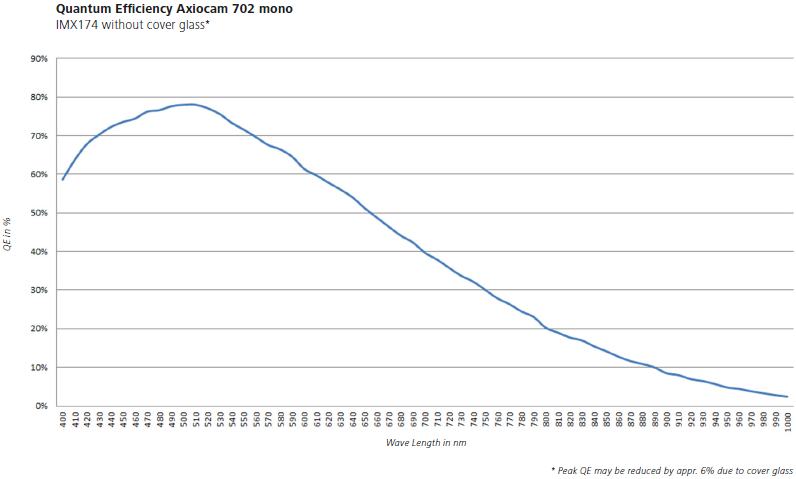
\includegraphics[width=7.0cm,height=7.0cm]{Figs/defectosZEISS/eficienciacuanticacamarazeiss.png}}{\caption{Gráfico de la eficiencia cuántica de la cámara monocromática del microscopio Aiocam 702 en función de la longitud de onda.}\label{fig:eficienciacuanticamara}}
		\ffigbox{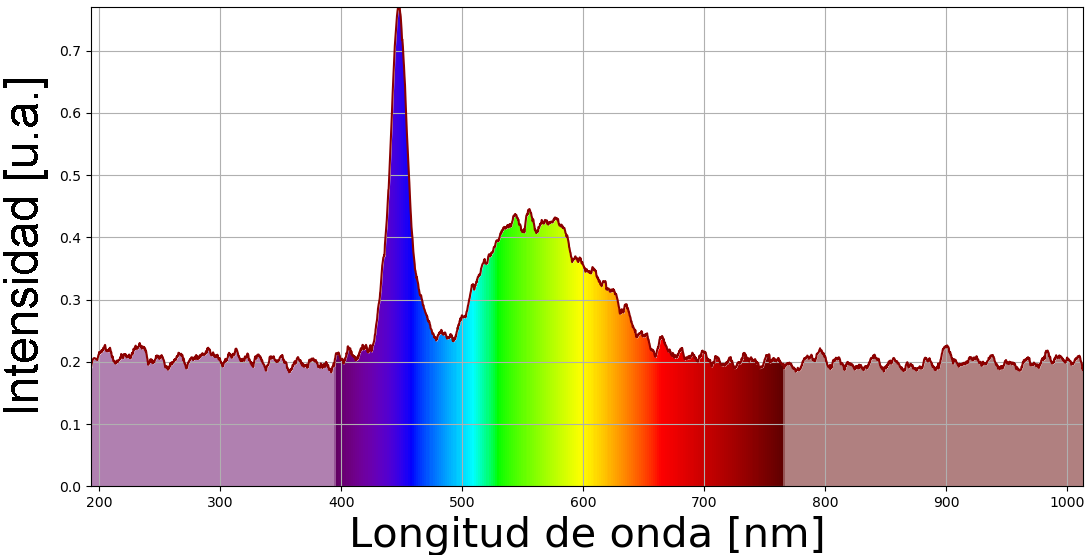
\includegraphics[width=7.0cm,height=7.0cm]{Figs/defectosZEISS/espectrolampZEISSacolor.png}}{\caption{Espectro de emisión de la fuente de luz del microscopio.}\label{fig:espectrolamparazeiss}}
	\end{floatrow}	
\end{figure}

\vspace{1.0cm}
\todo[inline]{mejorar esas figuras, no se ve nada y quedan desentonados}
\vspace{1.0cm}
\todo[inline]{cambiar escala de la longitud de onda a un rango mas chico, u.a no a.u. en castellano}
\vspace{1.0cm}
\todo[inline]{explicar que tipo de lampara es la del Zeiss}
\vspace{1.0cm}

La imagen completa de cada superficie exterior del filtro permitió:
\begin{itemize}
	\item Realizar un primer diagnóstico visual por imagen de la calidad óptica de construcción del filtro. 
	\item Observar la cantidad y tipo de defectos así como la densidad de los mismos.
	\item Determinar que ninguna de las dos superficies exteriores del filtro presentaba una cantidad mayor notable de defectos que la otra como se puede observar en las Figuras \ref{fig:supfiltrocondensador} y \ref{fig:supfiltroobjetivo}, por lo que el análisis individual de cada una de las bandas fue realizado sobre una de las caras únicamente.
	\item Obtener un mapa de los defectos con su ubicación precisa en la superficie del filtro.
\end{itemize}
\singlespacing
\subsection*{Adquisición de imágenes individuales de cada banda espectral}
\spacing{1.5}

\hspace{0.5cm}Para realizar una cuantificación de los defectos del filtro, se adquirieron imágenes individuales de cada banda espectral del filtro para una de las superficies exteriores del filtro. Para cada banda, se configuró la intensidad de la lámpara y el tiempo de integración de la cámara de forma tal de utilizar la mayor parte del rango dinámico de la cámara que se encuentra alrededor del 70 \% recomendado por el fabricante y de esta forma obtener la mejor calidad de imagen para cada banda y para su posterior análisis. 

\begin{figure}[!h]
	\centering
	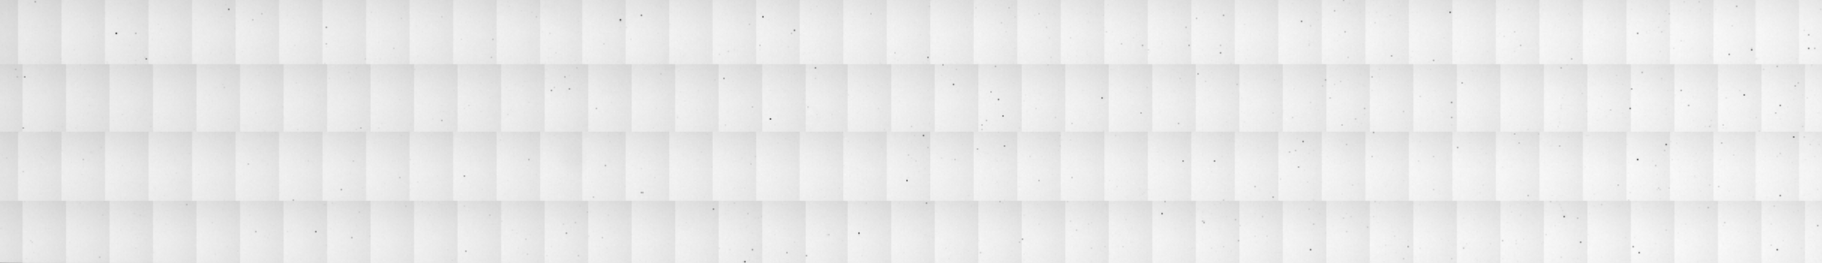
\includegraphics[width=1.0\textwidth,height= 5.0cm]{Figs/defectosZEISS/tilebandaroja.png}
	\caption{Imagen de la banda roja del filtro obtenida mediante un \textit{Tile scan}.}
	\label{fig:tilebandaroja}
\end{figure}

En la Figura \ref{fig:tilebandaroja} se muestra la adquisición de la banda roja obtenida mediante un \textit{tile scan} de 27.65 mm x 4.16 mm, intensidad de la lámpara configurada en 30\% y el tiempo de exposición de la cámara fue de 13 ms. En la sección de Resultados se muestran las imágenes de cada banda utilizadas para su análisis y su discusión.



\singlespacing
\section*{Pre-pocesamiento de las imágenes de cada banda espectral }
\spacing{1.5}

\vspace{1.0cm}
\todo[inline]{reescribir oracion de abajo}
\vspace{1.0cm}
\todo[inline]{xq necesito cada etapa, qué hago cone l pre-procesamiento y después con el resto}
\vspace{1.0cm}

\hspace{0.5cm}El análisis de las imágenes fue realizado sobre cada \textit{tile} individual del barrido completo de una banda, dado que su tamaño típico es de 3 MB por lo que el procesamiento en la computadora es mucho más rápido que el de analizar las imágenes de una banda completa, de tamaños típicos de 1 GB ó del filtro completo que tienen más de 5 GB.

El pre-procesamiento de las imágenes de cada banda espectral consiste en la corrección en las imágenes de la iluminación no uniforme del microscopio que se realiza normalizando las imágenes individuales del barrido con una imagen de fondo. Este preprocesamiento consiste de dos pasos:
\begin{enumerate}
	\item  Se construyó cada imagen de fondo a partir de tomar la mediana de cada píxel de todas las imágenes adquiridas en el \textit{tile scan} \cite{Nordenfelt}. Esta imagen de fondo contiene la información de cada píxel que está presente en todas las imágenes adquiridas en el barrido completo de una banda y debe ser generada para cada banda en particular, considerando que cada una de ellas fue adquirida en ciertas condiciones de intensidad de la fuente de luz y del tiempo de integración de la cámara. 
	
	\begin{figure}[H]
		\centering
		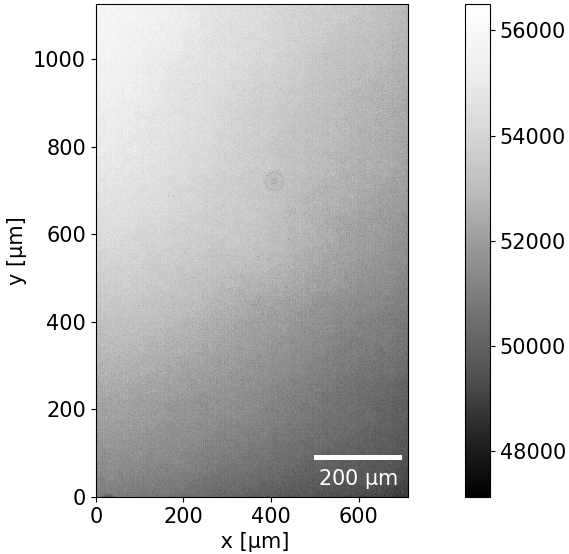
\includegraphics[scale=0.2]{Figs/defectosZEISS/bg_celeste.png}
		\caption{Imagen de fondo de la banda celeste del filtro obtenida tomando la mediana para cada píxel de todas las imágenes del barrido.}
		\label{fig:bgcel}
	\end{figure}
	\hspace{0.5cm}En la Figura \ref{fig:bgcel} se muestra la imagen de fondo adquirida para la banda celeste, cuya intensidad de la fuente de luz fue configurada en 30$\%$ y el tiempo de integración de la cámara fue de 40 ms. Los dos discos concéntricos que se observan en la imagen son resultado de un defecto en algún componente óptico del microscopio, ya advertido por otros usuarios del equipo. El código escrito de la construcción de la imagen de fondo se puede ver en el siguiente link: \href{https://github.com/jrr1984/defects_analysis/blob/master/MAIN/bg.py}{\faGithub}.
	
	\vspace{1.0cm}
	\todo[inline]{aclarar al principio de todo que el simolito es un link a github}
	\vspace{1.0cm}
	
	\item Con la imagen de fondo ya construida, se normalizaron las imágenes originales del barrido completo de una banda. En las Figuras \ref{fig:sinnorm} y \ref{fig:connorm} se muestra una imagen de una \textit{tile} individual del barrido de la banda del NIR antes y después de ser normalizada, respectivamente. El código escrito de este paso se puede ver en el siguiente link: \href{https://github.com/jrr1984/defects_analysis/blob/master/MAIN/bg_normalization.py}{\faGithub}.
	
	\todo{el defecto de la imagen de fondo puede ser la reflexión del objetivo}
	\begin{figure}[H]
		\begin{floatrow}
			\ffigbox{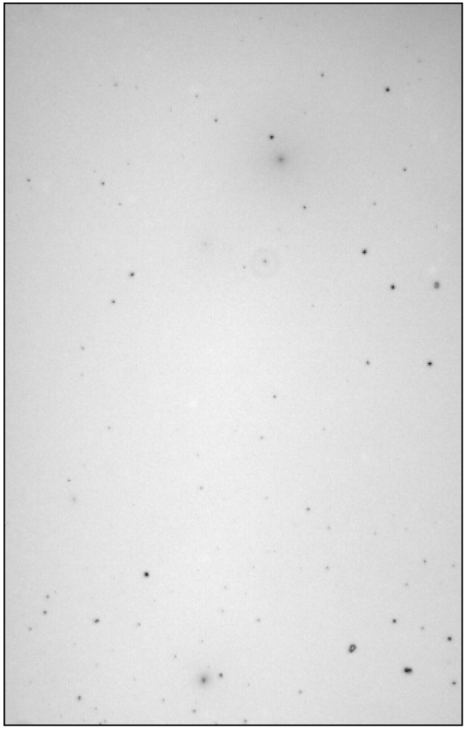
\includegraphics[width=7.0cm,height=10.0cm]{Figs/defectosZEISS/Experiment-11_m001_ORG.png}}{\caption{Imagen original de una \textit{tile} del barrido completo de la banda del NIR. }\label{fig:sinnorm}}
			\ffigbox{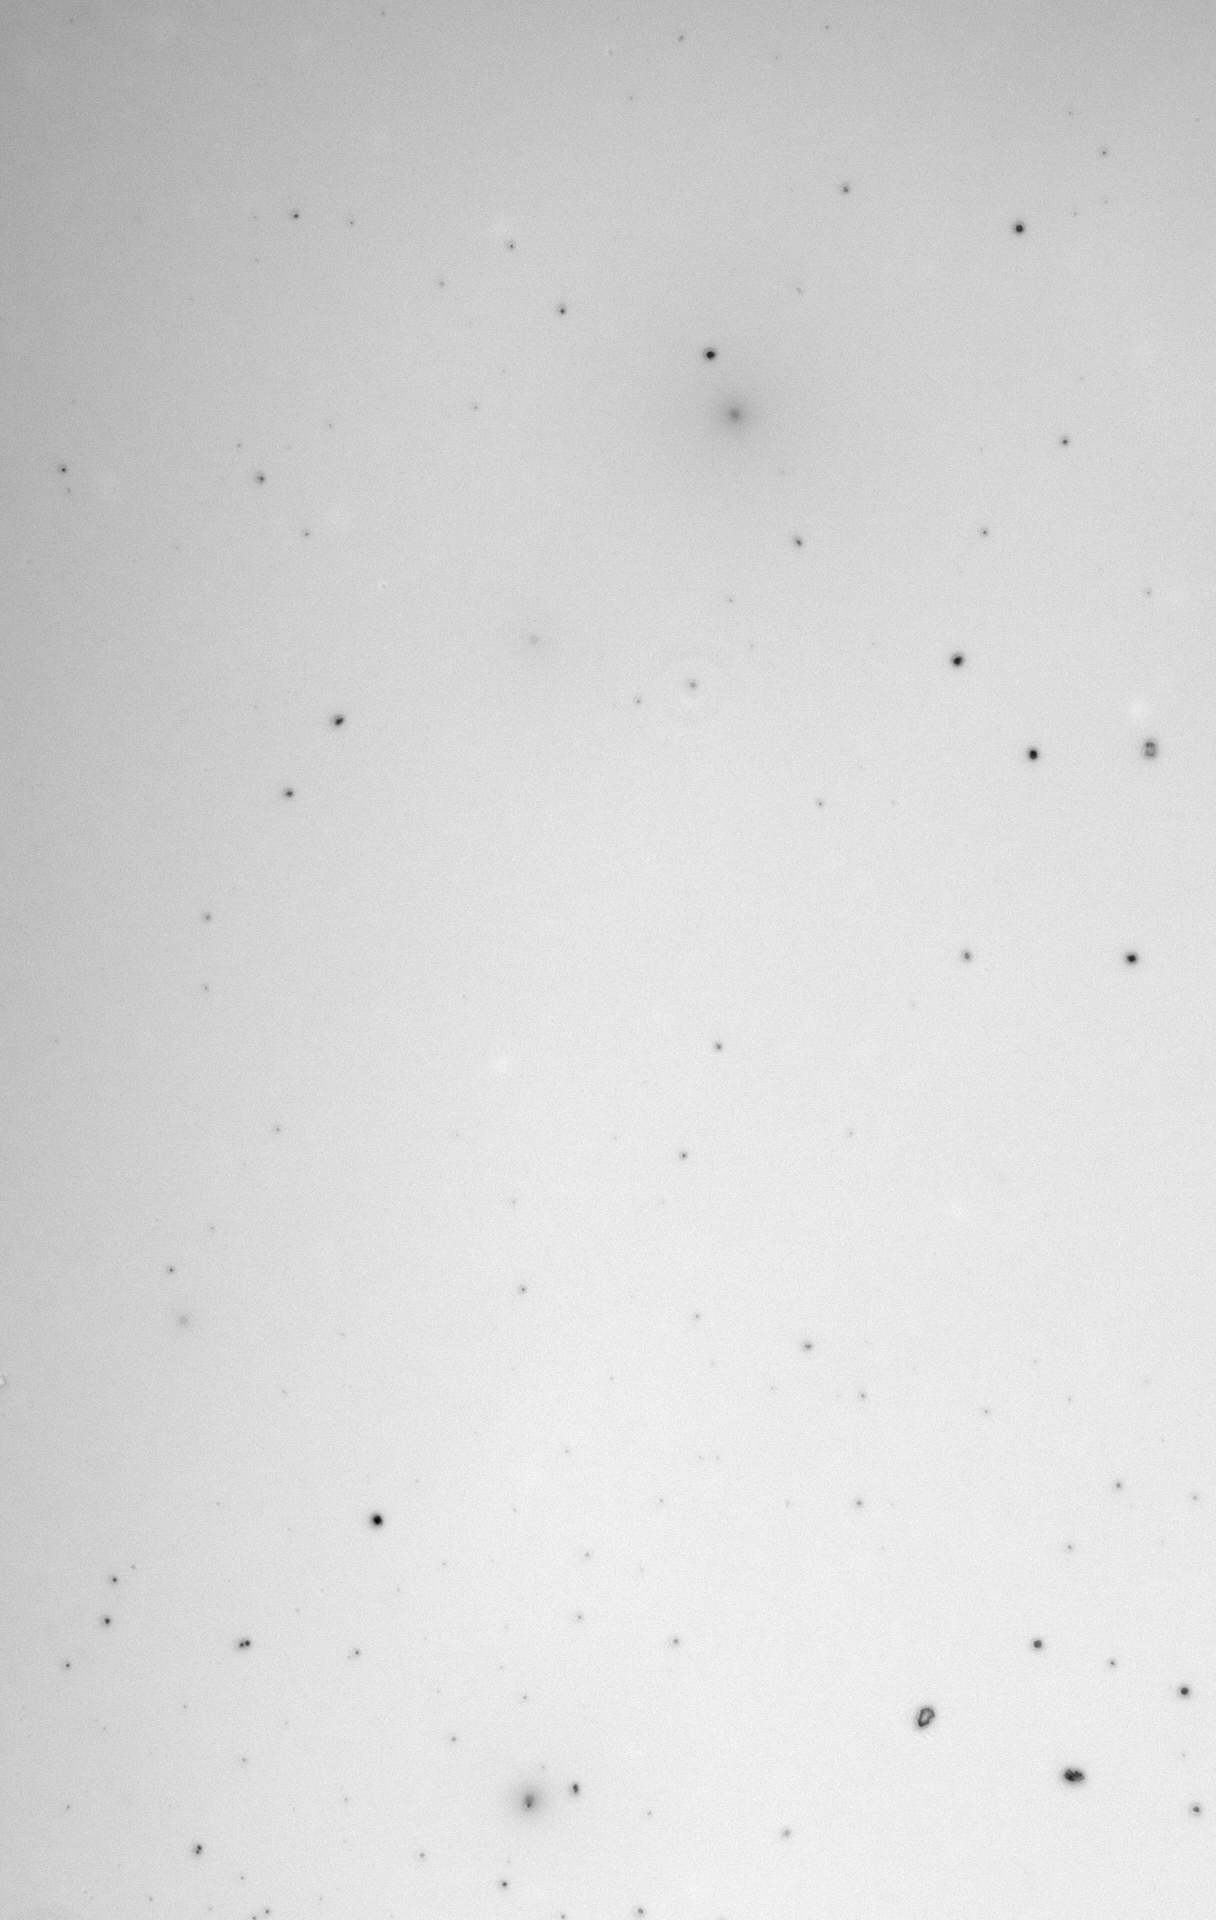
\includegraphics[width=7.0cm,height=10.0cm]{Figs/defectosZEISS/normNIR_1.png}}{\caption{Imagen normalizada a partir de la imagen de fondo.}\label{fig:connorm}}
		\end{floatrow}
	\end{figure}
	
	\vspace{1.0cm}
	\todo[inline]{restar las dos imágenes, mejorar eso.}
	\vspace{1.0cm}
	
\end{enumerate}

\singlespacing
\section*{Algoritmo de detección de los defectos}
\spacing{1.5}

\hspace{0.5cm}Con las imágenes pre-procesadas la detección de los defectos fue realizada utilizando algoritmos de procesamientos de imágenes. El algoritmo consistió de los siguientes pasos:
\begin{enumerate}
	\item Se determina el valor de intensidad umbral (en adelante, \textit{threshold}) a partir del cual se distingue entre un defecto en la región de la imagen que se \textit{foreground} y el fondo de la imagen (\textit{background}). %Iterando sobre los conjuntos completos completos de \textit{tiles} de cada banda se determinó que el t
\end{enumerate}





\singlespacing
\section*{Resultados del algoritmo de detección de los defectos}
\spacing{1.5}


\hspace{0.5cm}Los resultados del algoritmo de detección de los defectos son guardados en un archivo \textit{pickle}\footnote{Con el módulo \textit{pickle} de python se puede serializar cualquier tipo de objeo de python y guardarse en un archivo \textit{pickle}, de extensión .pkl, que resulta muy eficiente tanto en su escritura como en su lectura.} que puede ser abierto y manipulados sus datos con la librería \textit{pandas} de python en el marco de lo que se conoce como un \textit{pandas dataframe} que no es más que un objeto de python que permite una manipulación de los datos muy eficiente. A continuación se muestra un resumen de los resultados para cada banda espectral del filtro.

\singlespacing
\subsection*{Defectos de la banda NIR}
\spacing{1.5}


\begin{figure}[H]
	\centering
	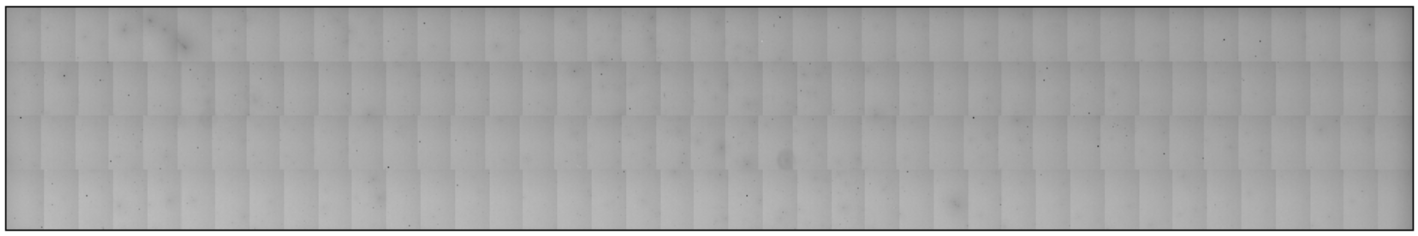
\includegraphics[width=1.0\textwidth,height= 5.0cm]{Figs/resultados_defectos/banda_nir.png}
	\caption{\textit{tile scan} obtenido de la banda NIR de 26.37 mm x 4.16 mm.}
	\label{fig:bgcel}
\end{figure}


\begin{figure}[H]
	\centering
	\includegraphics[width=1.0\textwidth,height= 5.0cm]{Figs/resultados_defectos/tabla_nir.png}
	\caption{Tabla del resumen de resultados del dataframe de la banda NIR.}
	\label{fig:bgcel}
\end{figure}

\singlespacing
\subsection*{Defectos de la banda Roja}
\spacing{1.5}


\begin{figure}[H]
	\centering
	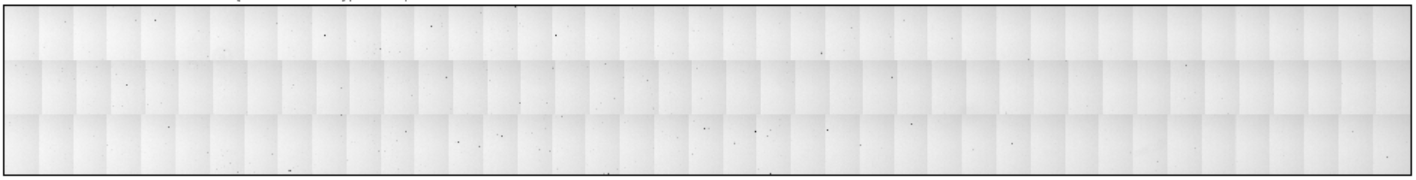
\includegraphics[width=1.0\textwidth,height= 5.0cm]{Figs/resultados_defectos/banda_roja.png}
	\caption{\textit{tile scan} obtenido de la banda roja de 26.37 mm x 3.15 mm.}
	\label{fig:bgcel}
\end{figure}


\begin{figure}[H]
	\centering
	\includegraphics[width=1.0\textwidth,height= 5.0cm]{Figs/resultados_defectos/tabla_roja.png}
	\caption{Tabla del resumen de resultados del dataframe de la banda roja.}
	\label{fig:bgcel}
\end{figure}






El código de este capítulo fue escrito utilizando python 3.6.7 y paquetes numpy 1.17.3, scikit-image 0.16.2 y matplotlib 3.1.2, entre otros.


\vspace{1cm}
\todo[inline]{estimacion de errores, ROI estimacion de falsos positivos falsos negativos tasa de error del sistema, por inspeccion visual nomas}
\vspace{1cm}


\vspace{1cm}
\todo[inline]{ver imagenes y cuantificar cuantos defectos de los mas chicos no agarra, se hace a ojo si o si, revisar banda completa tomando nota de defectos reales vs defectos encontrados y cuantificarlo de alguna manera}
\vspace{1cm}

\vspace{1cm}
\todo[inline]{diagrama de flujo para el algoritmo de deteccion}
\vspace{1cm}

\vspace{1cm}
\todo[inline]{poner grafico del espectro de la lampara con colores facha y explicar que tipo de lampara es, escuchar audio hernan}
\vspace{1cm}

%\chapter{Spectral GUI y software del primer prototipo: Integración clases del espectrómetro y de los motores de thorlabs -Implementación con Multithreading}

\chapter{Desarrollo XZStage y calibración - Desarrollo del software integrando el arduino con algoritmos asincrónicos}

\singlespacing
\chapter{Microespectrómetro}
\spacing{1.5}

\hspace{0.5cm}En este capítulo se describe el montaje y la caracterización de un microespectrómetro utilizado para caracterizar espectralmente los defectos del filtro.



\singlespacing
\section*{Diseño óptico del microespectrómetro}
\spacing{1.5}

\singlespacing
\section*{Montaje y alineación preliminar del microespectrómetro}
\spacing{1.5}

\singlespacing
\section*{Foco y resolución espacial del microespectrómetro}
\spacing{1.5}

\hspace{0.5cm}Para poner en foco el microespectrómetro sobre la cara externa del filtro más cerca al objetivo, se buscó el mínimo de la resolución espacial.

La resolución espacial se obtiene a partir del ajuste de las mediciones de una transición banda-cromo.

Para no alargar el tiempo de duración de las mediciones se mapeó el espectrómetro con la cámara. De lo contrario el único feedback que se tiene para saber si se está en una banda o en el cromo es la medición del espectro.

En consecuencia se conectó la fibra óptica montada sobre el cage destinado a medir con el espectrómetro, a la fuente de luz y por reflexión se observó en la adquisición en vivo de la cámara en qué posición de la imagen se observaba el haz de luz reflejado. Se centró dicho haz al centro de la cámara y de esa forma se determinó que el centro de la cámara está asociado con la medición efectiva del microespectrómetro. Se hace notar que la cámara no se encuentra en foco todavía, solo fue puesta aproximadamente a la misma distancia focal que la lente de tubo.

El setup para realizar este mapeo es el siguiente:
\begin{figure}[H]
	\centering
	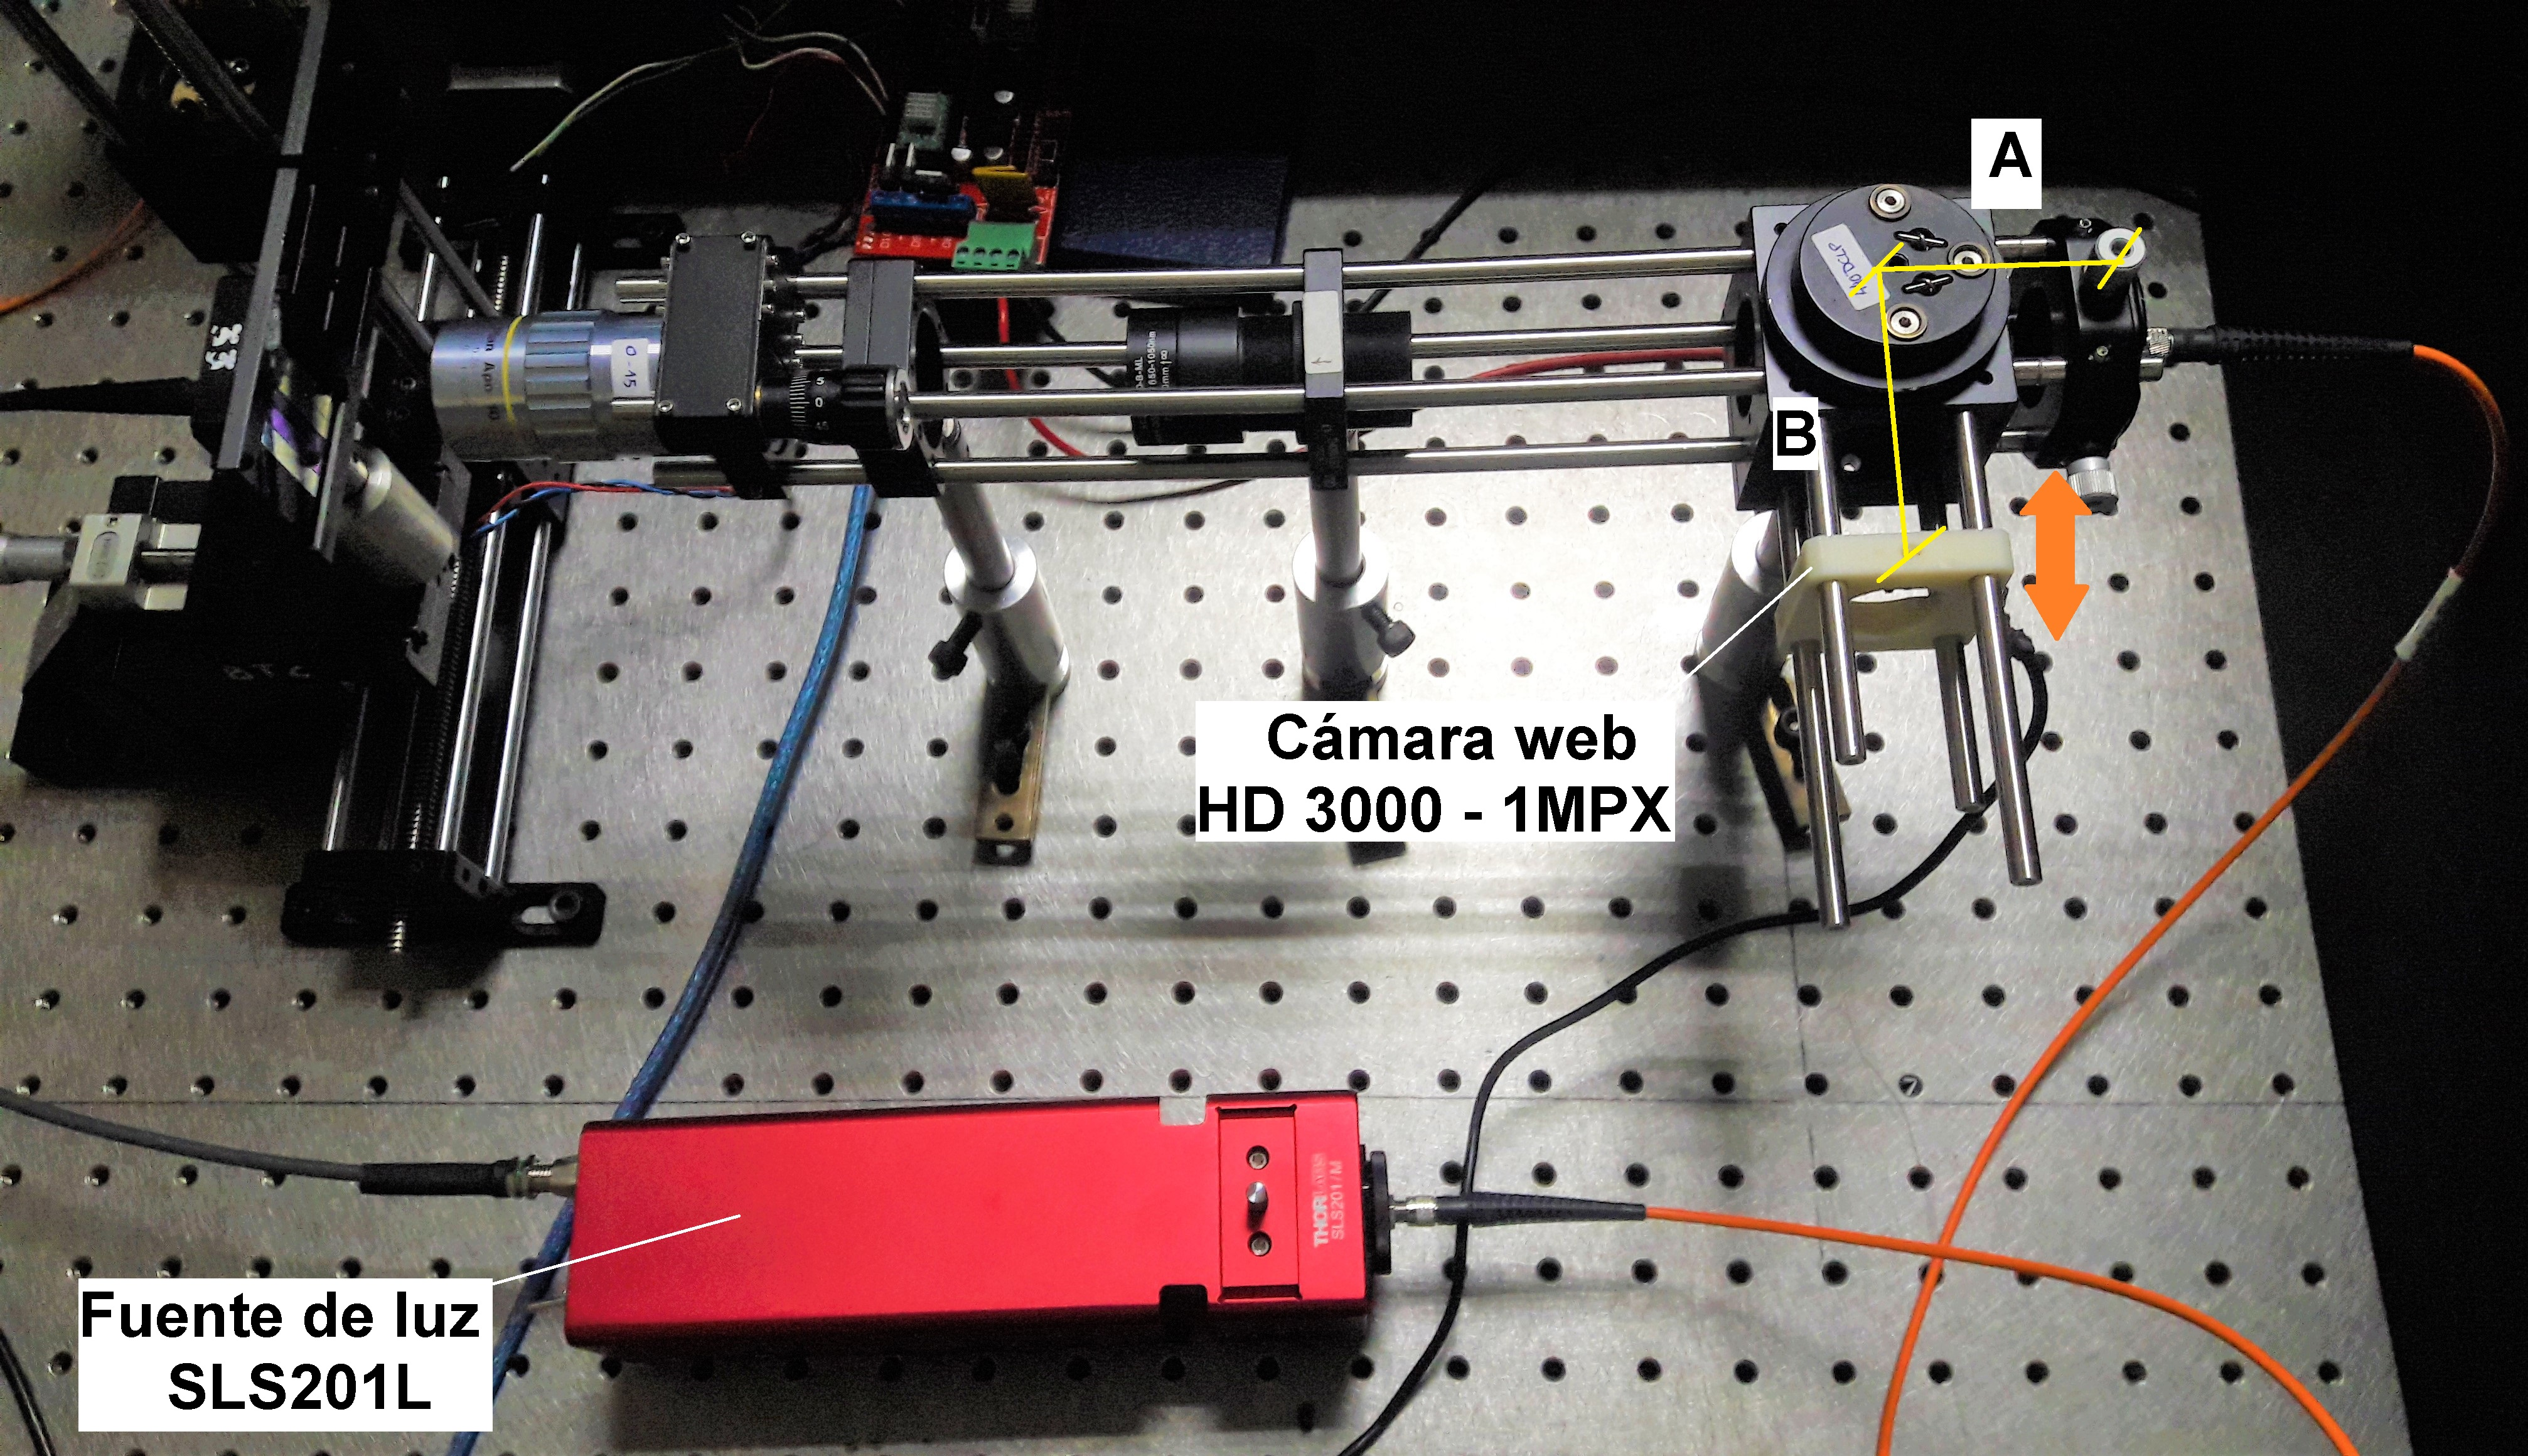
\includegraphics[scale=0.1]{Figs/microespectrometro/mapespeccam.jpg}
	\caption{Setup para mapear el espectrómetro con la cámara.}
	\label{fig:bgcel}
\end{figure}


Con los tornillos de la tapa de arriba del beamsplitter se puede ajustar en altura el beamsplitter para poder observar en el centro de la cámara la medición del espectrómetro.
\begin{figure}[H]
	\centering
	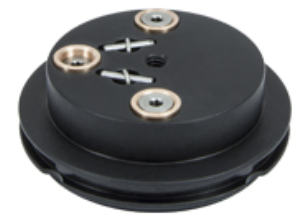
\includegraphics[scale=0.5]{Figs/microespectrometro/b4c.png}
	\caption{Tapa de arriba del beamsplitter.}
	\label{fig:bgcel}
\end{figure}


\begin{figure}[H]
	\centering
	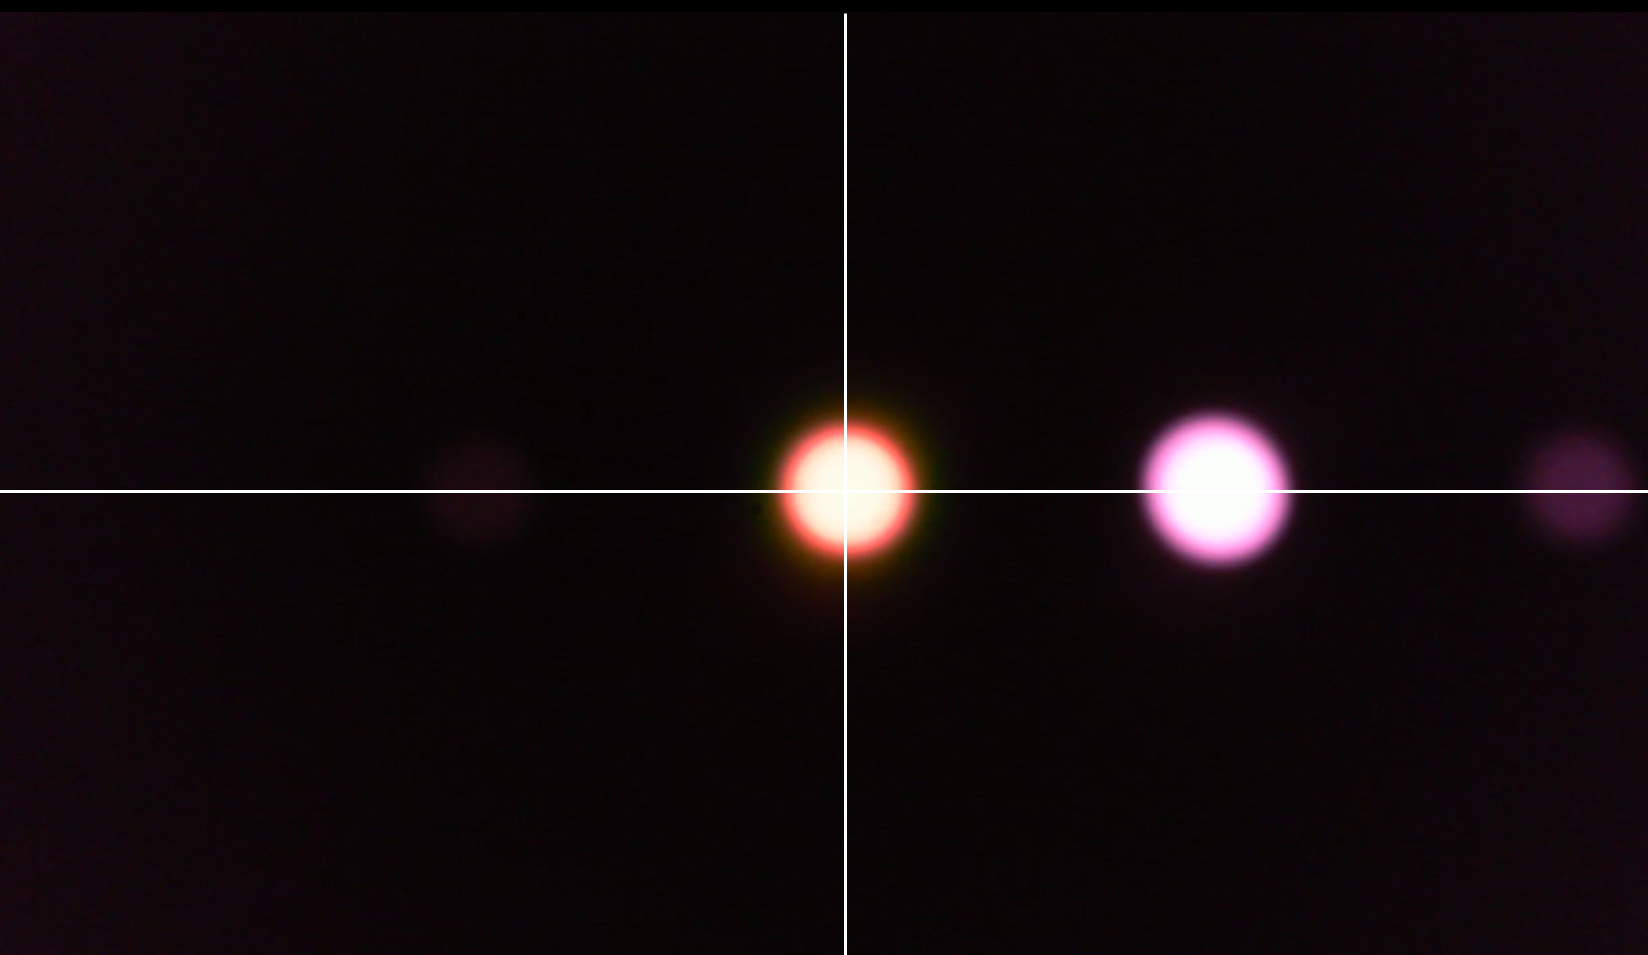
\includegraphics[scale=0.5]{Figs/microespectrometro/mapspectrometrocamera.png}
	\caption{Visualización en la cámara de la reflexión del filtro de la iluminación.}
	\label{fig:bgcel}
\end{figure}


No se tocó ni la cámara ni ninguna parte del setup a partir de ese momento para no perder este mapeo, a pesar de que la cámara no se encuentre perfectamente en foco (no hace falta probablemente poner una imagen de la cámara mostrando que no está en foco..), es decir que la imagen no se vea del todo nítida.
Luego se puso en foco el microespectrómetro.



\begin{figure}[H]
	\centering
	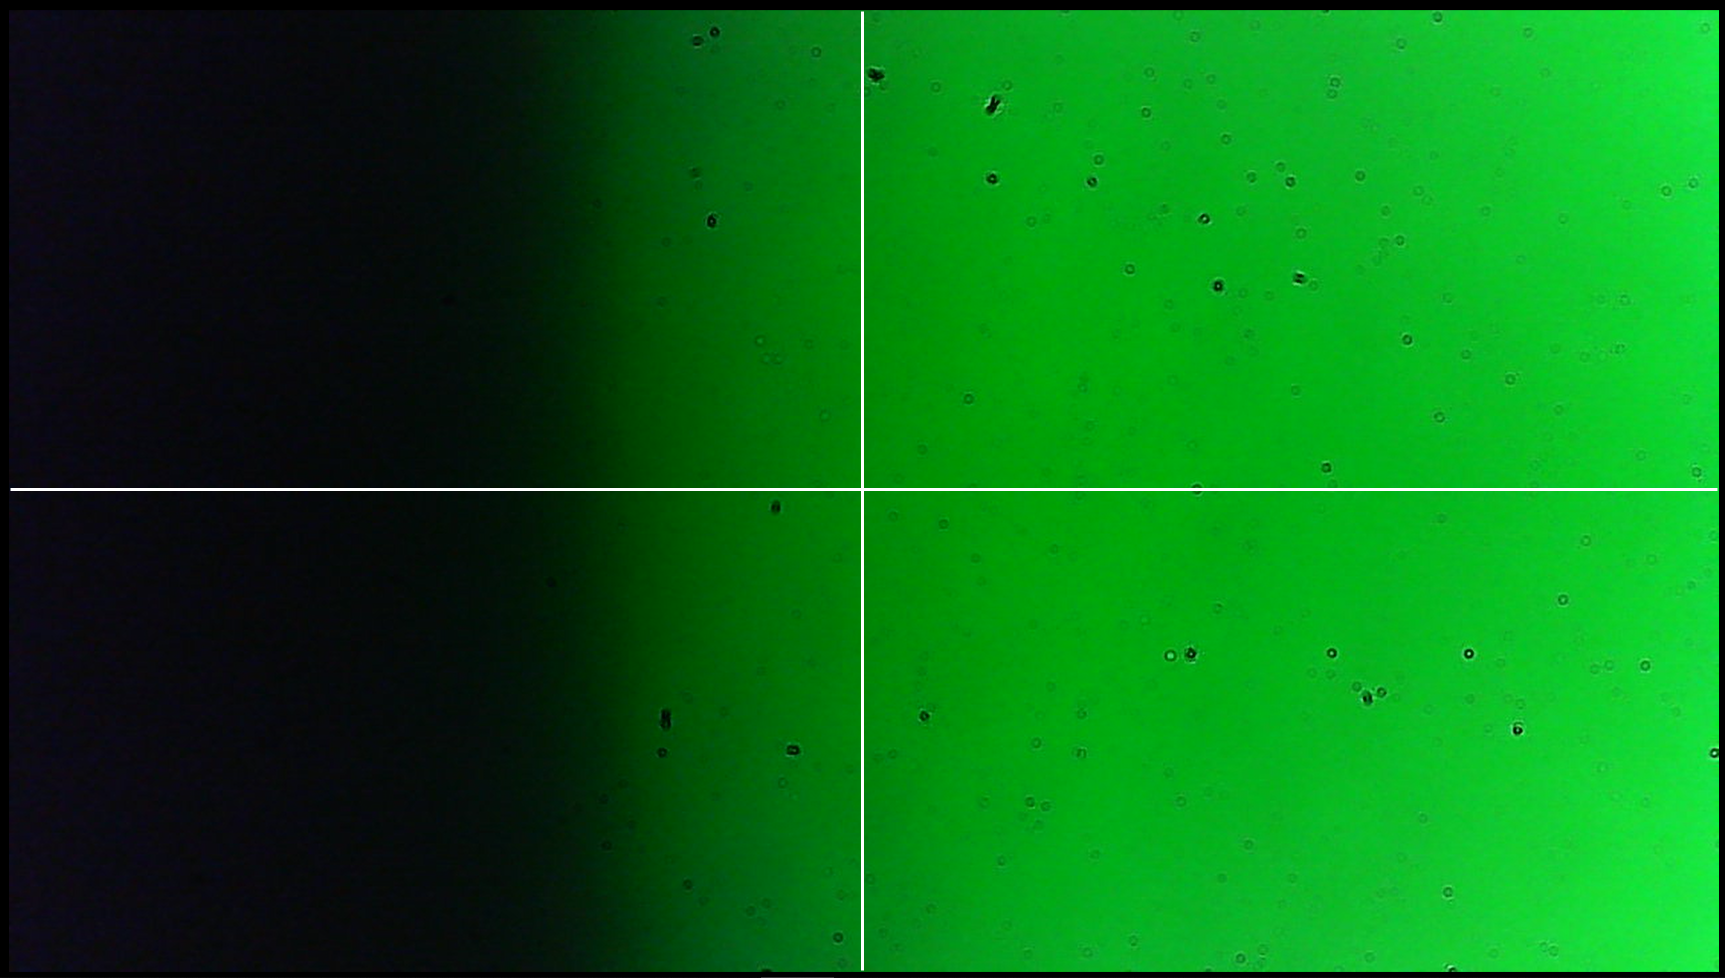
\includegraphics[scale=0.5]{Figs/microespectrometro/medtransicion.png}
	\caption{Visualización en la cámara de la reflexión del filtro de la iluminación.}
	\label{fig:bgcel}
\end{figure}


durante el experimento se tiene el feedback de cutelog:

\begin{figure}[H]
	\centering
	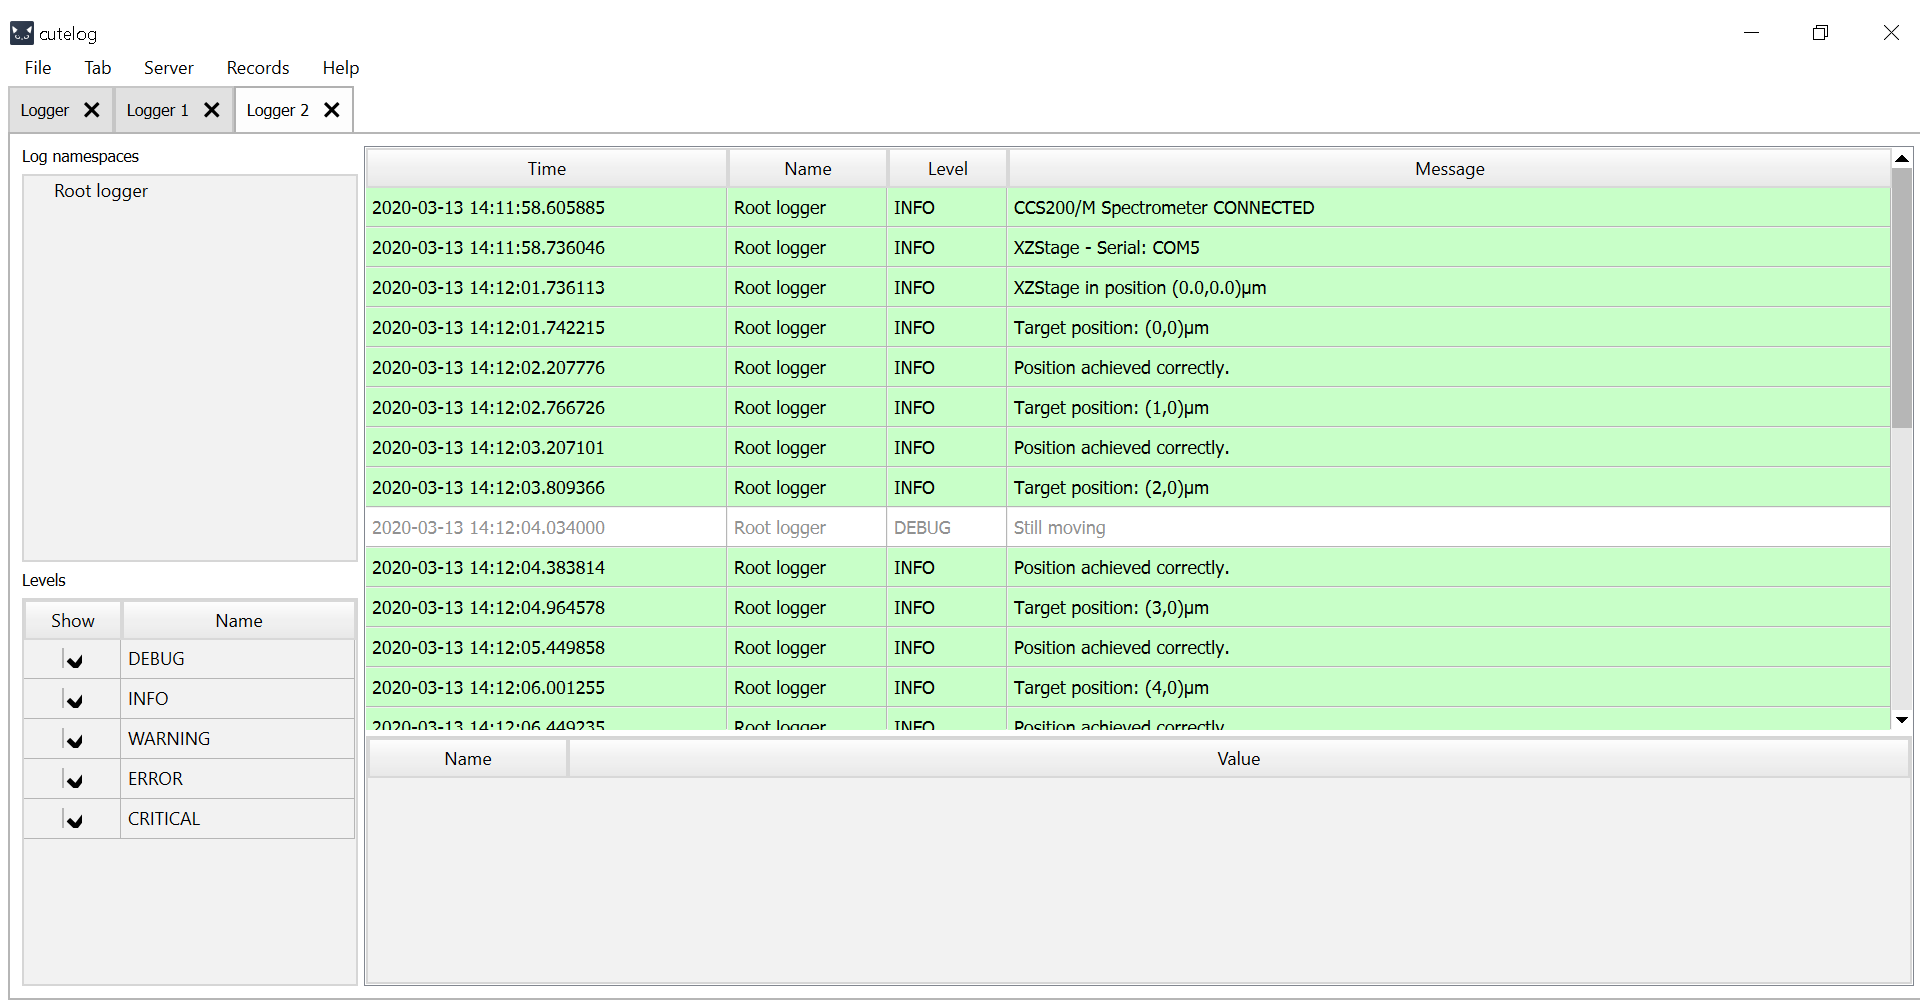
\includegraphics[scale=0.5]{Figs/microespectrometro/cutelog.png}
	\caption{Visualización en la cámara de la reflexión del filtro de la iluminación.}
	\label{fig:bgcel}
\end{figure}


\begin{figure}[H]
	\centering
	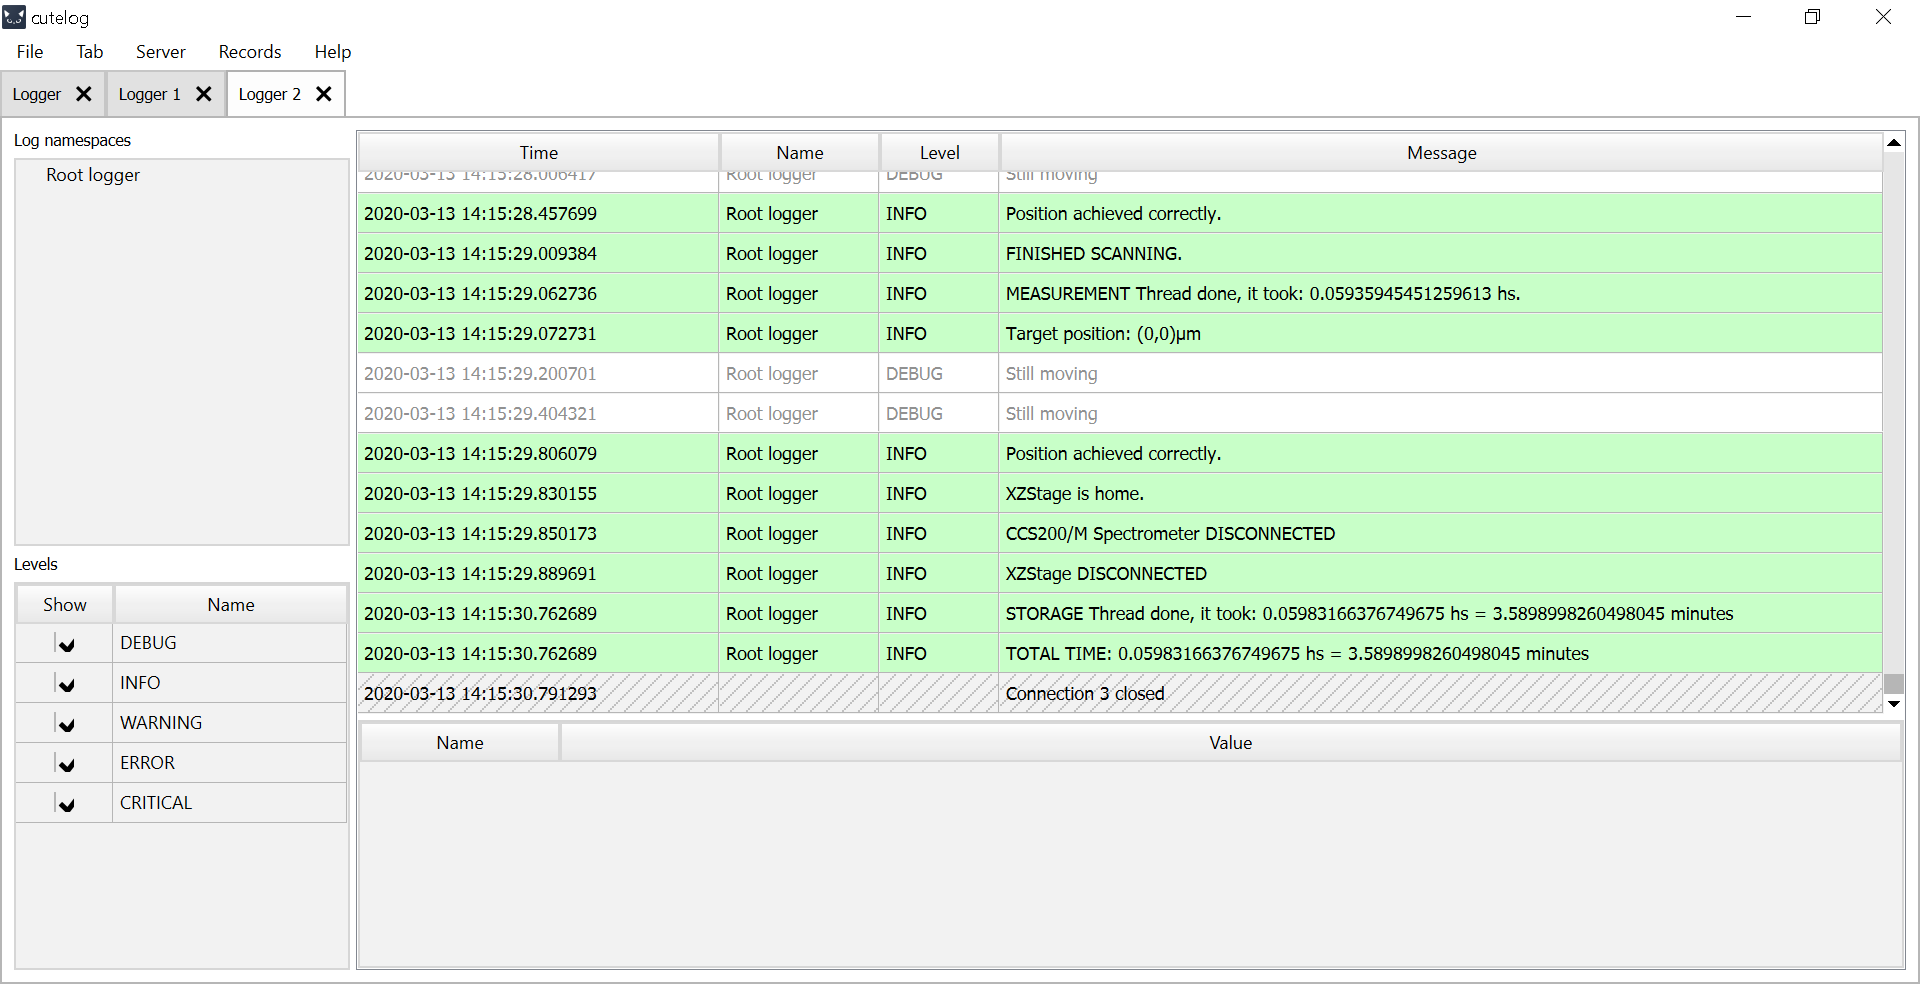
\includegraphics[scale=0.5]{Figs/microespectrometro/fincutelog.png}
	\caption{Visualización en la cámara de la reflexión del filtro de la iluminación.}
	\label{fig:bgcel}
\end{figure}


Las mediciones son ajustadas en matlab con una función error:
\begin{equation}
	(a/2)*erfc(sqrt(2)*(x-b)/c)
\end{equation}

\begin{figure}[H]
	\centering
	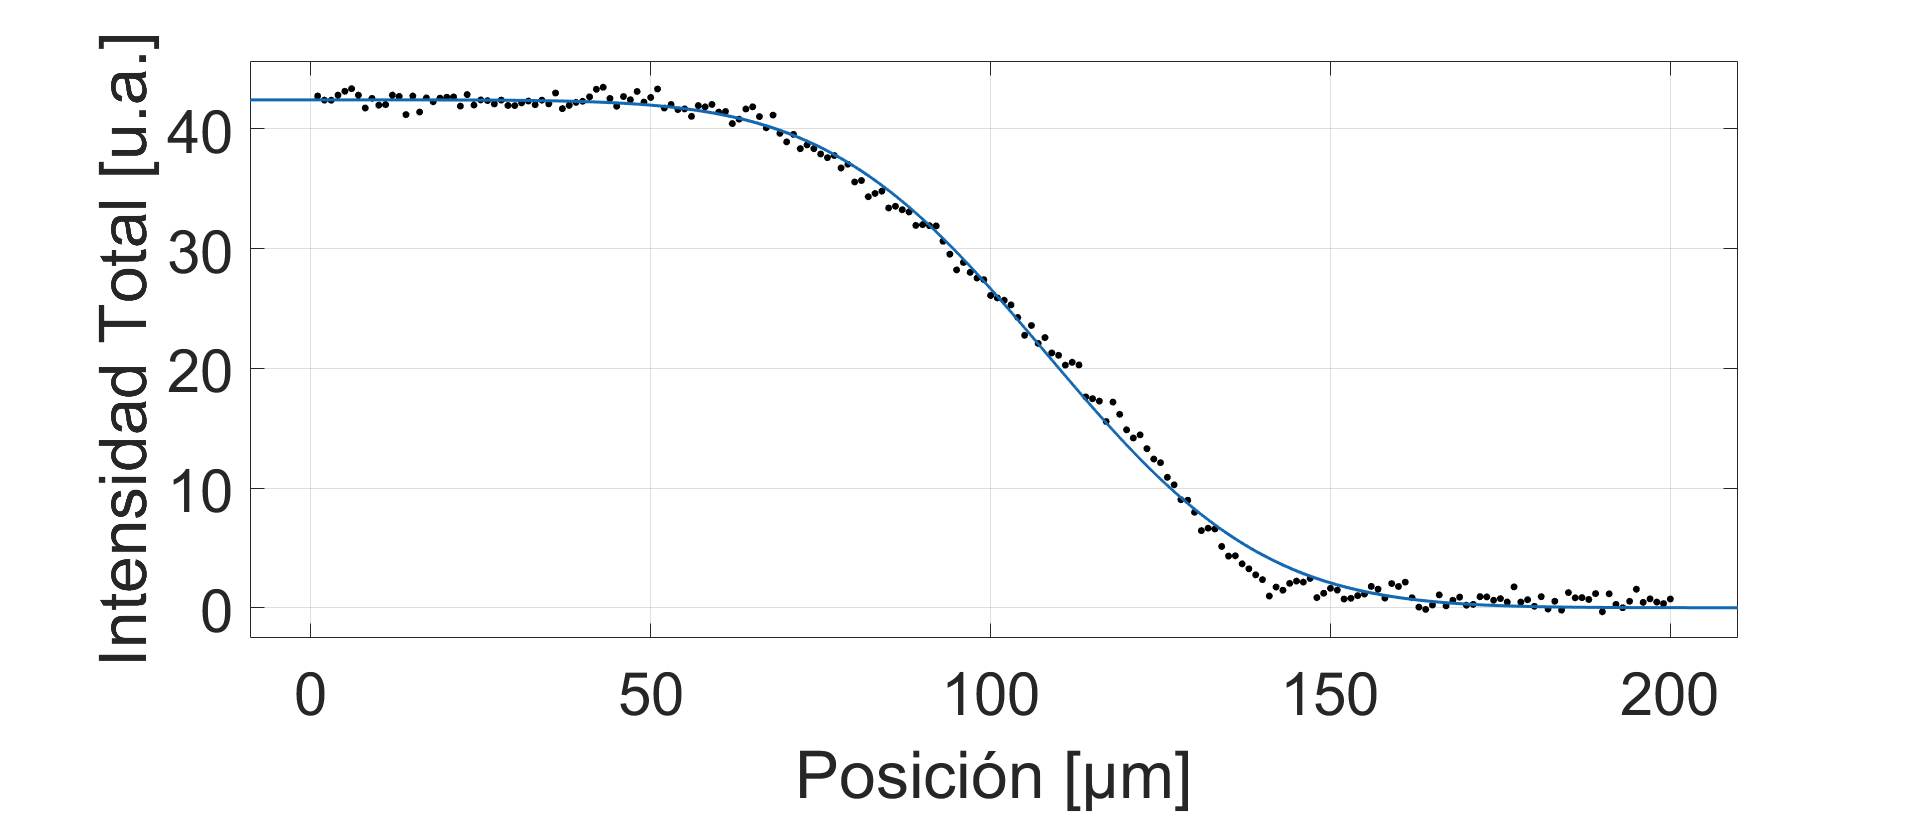
\includegraphics[scale=0.3]{Figs/microespectrometro/fit0.png}
	\caption{Visualización en la cámara de la reflexión del filtro de la iluminación.}
	\label{fig:bgcel}
\end{figure}

Resultados del ajuste:

General model:\par
$f(x) = (a/2)*erfc(sqrt(2)*(x-b)/c)$ \par
Coefficients (with 95$\%$ confidence bounds): \par
$a =       42.43  (42.2, 42.66)$\par
$b =       108.2  (107.8, 108.7)$\par
$c =       50.46  (49.25, 51.68)$\par

Goodness of fit:\par
SSE: 151.1\par
R-square: 0.9976\par
Adjusted R-square: 0.9976\par
RMSE: 0.8758\par

Luego moviendo la perilla del SM1Z para cambiar la distancia entre el objetivo y el filtro se repite la medición.


Comentar bien la siguiente foto, poner en la imagen que distancia se está variando, ettc
\begin{figure}[H]
	\centering
	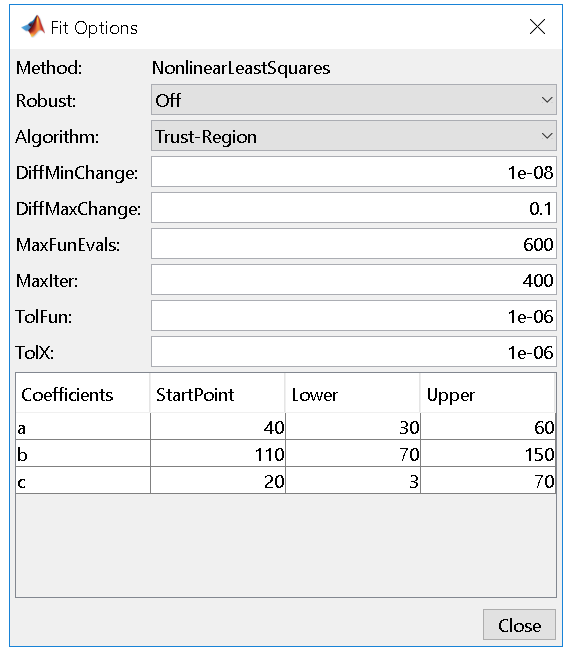
\includegraphics[scale=0.4]{Figs/microespectrometro/refinacionparam.png}
	\caption{Visualización en la cámara de la reflexión del filtro de la iluminación.}
	\label{fig:bgcel}
\end{figure}


Para hacer el ajuste se refinan los parámetros del modelo:

\begin{figure}[H]
	\centering
	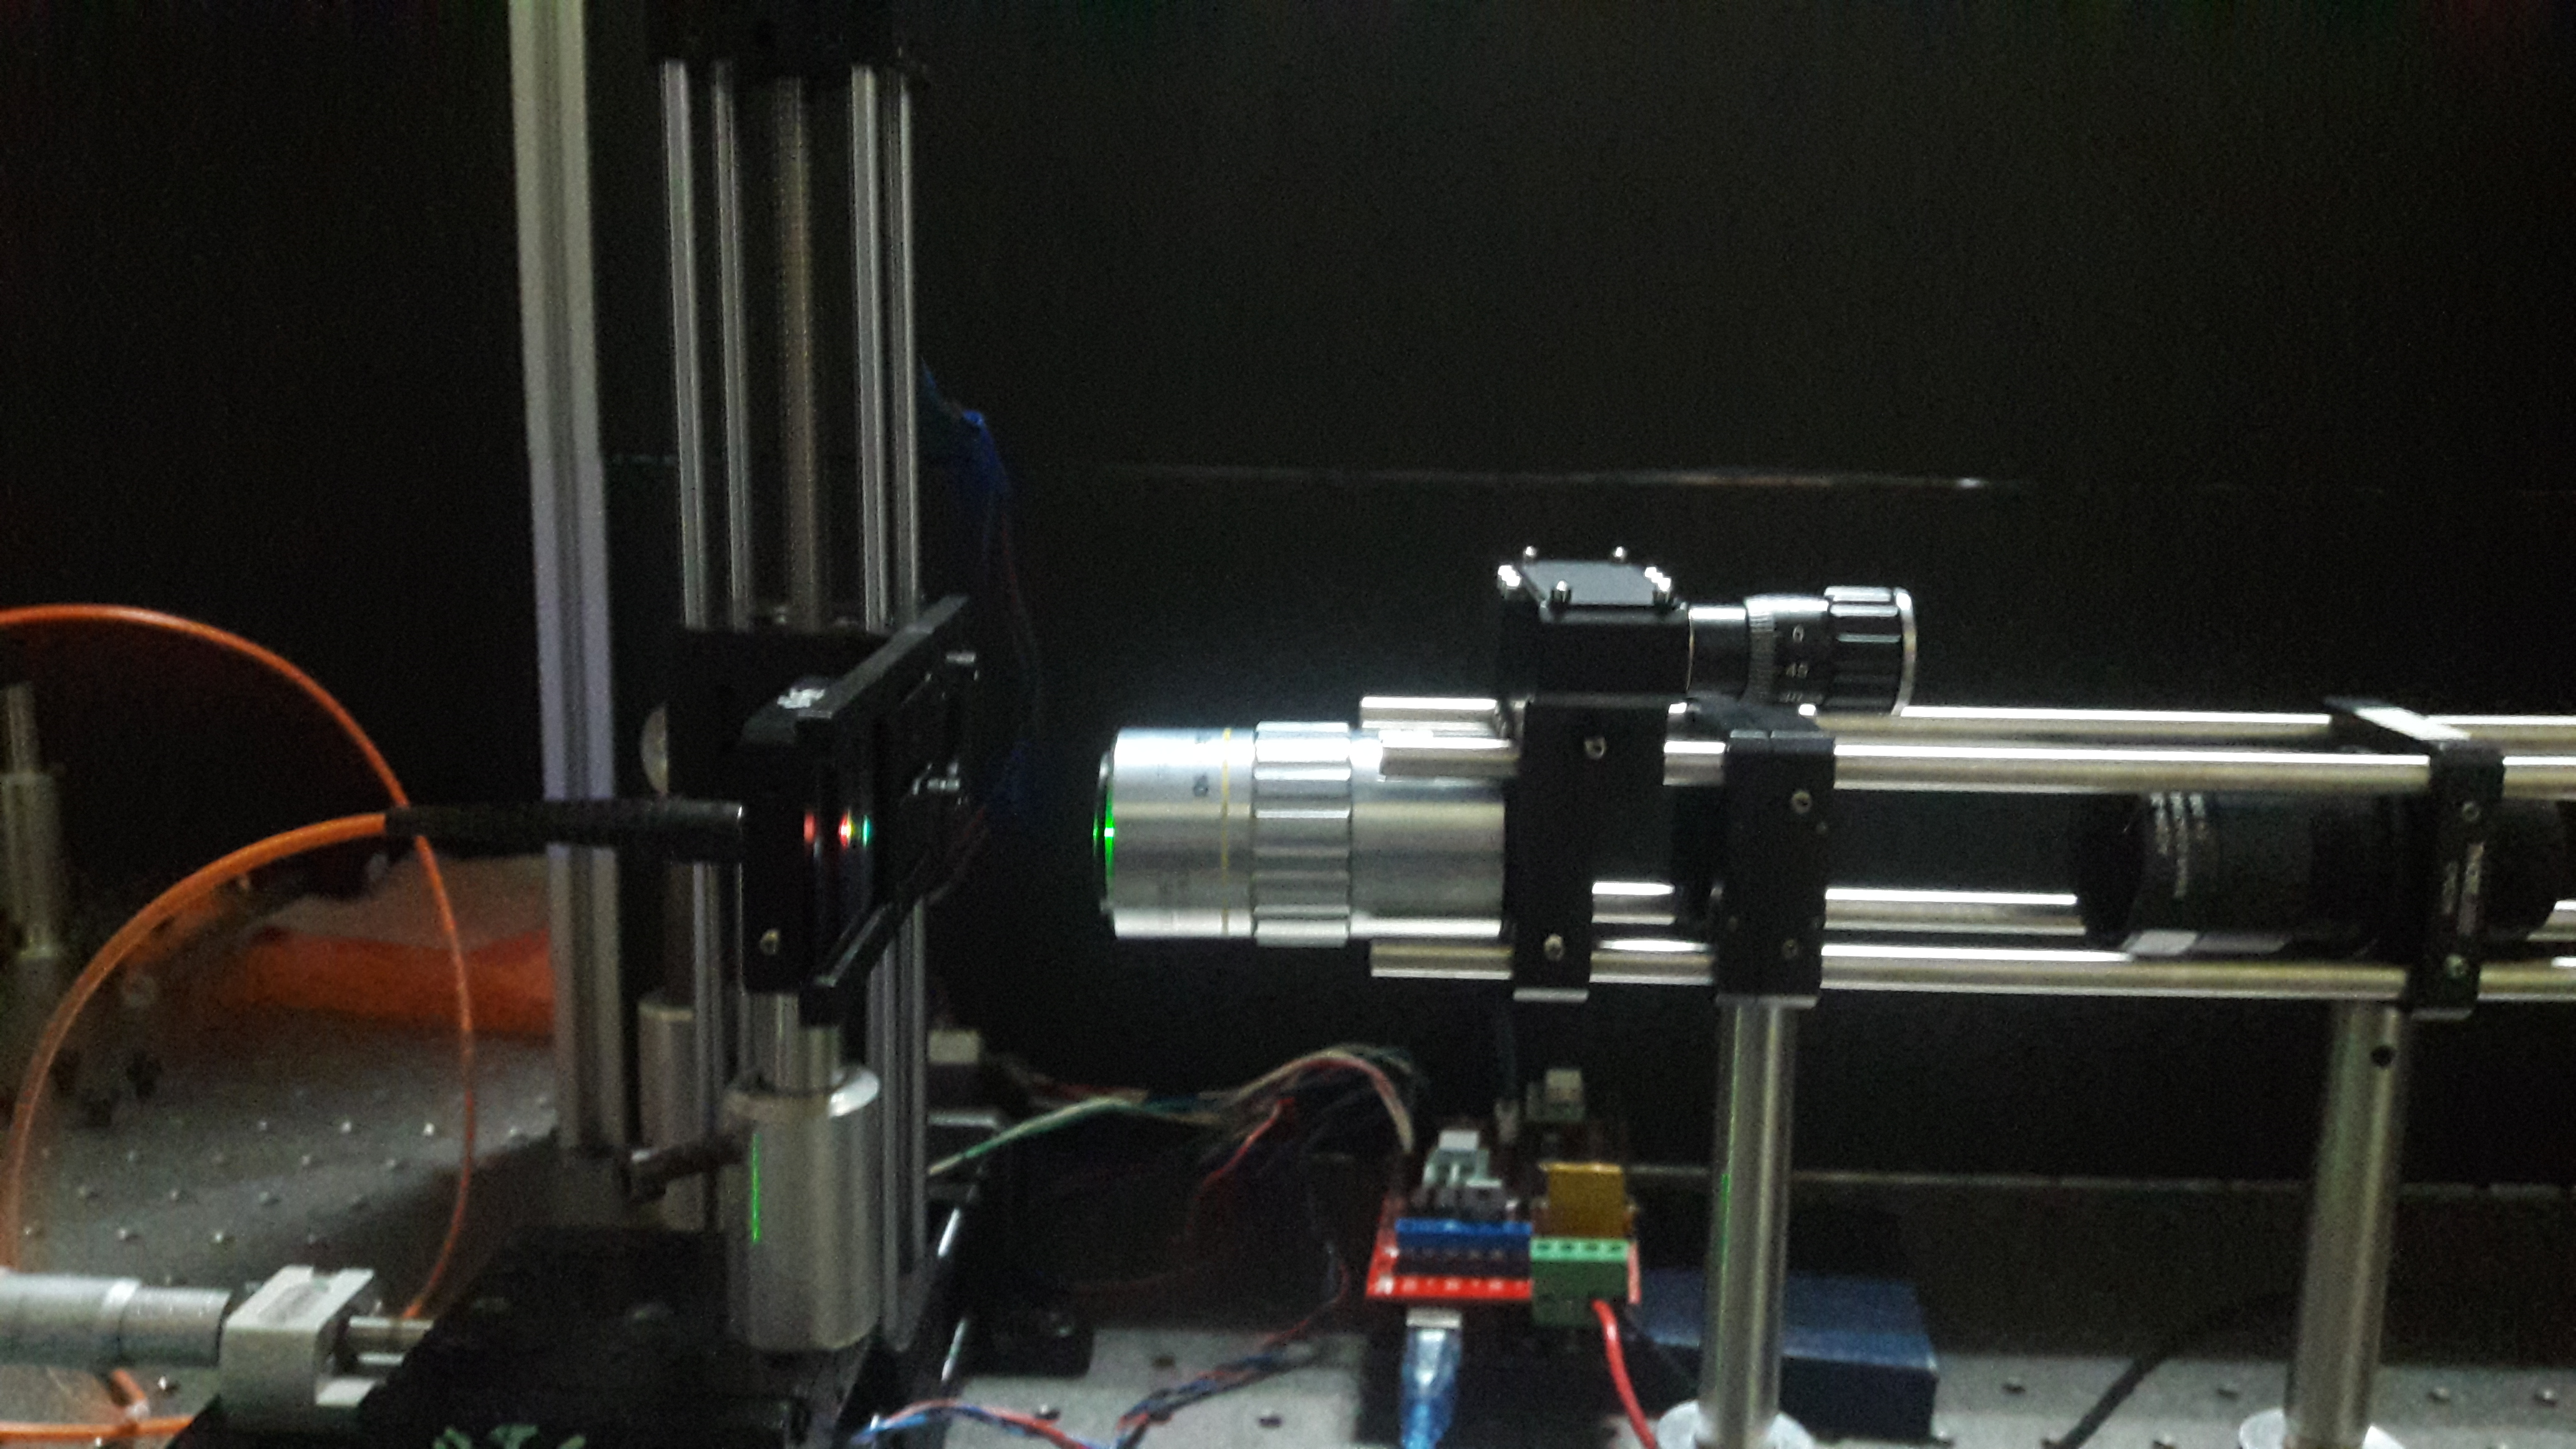
\includegraphics[scale=0.1]{Figs/microespectrometro/sm1zcambio.jpg}
	\caption{Visualización en la cámara de la reflexión del filtro de la iluminación.}
	\label{fig:bgcel}
\end{figure}


La idea es poner en foco el espectrómetro en alguna región del filtro, enfocar luego la cámara y después al mover el filtro a alguna otra región, tan solo hay que poner en foco el 'sistema' mirando la cámara. Al mismo tiempo si se quiere se puede volver a repetir el procedimiento de buscar el mínimo.


Gráfico de poner en foco el microespectrómetro: (19 de marzo)

mediciones guardadas en: data mediciones, simultaneidad, foco.

vamos recorriendo horario en pasos de 50 micrones en el SM1Z.
mediciones que consisten en un barrido de 80 micrones de largo, con pasos de 1 micron.. esto en la stage


RESULTADOS:

Z                  RESOLUCIÓN

0                  12.46 dudoso?

-50               13.5

-100             13.12

-150              12.87

-200              11.29



\singlespacing
\section*{Integración de una cámara web}
\spacing{1.5}

\singlespacing
\subsection*{Mapeando el espectrómetro con la cámara}
\spacing{1.5}




\chapter{Conclusiones}

\chapter{Trabajo a futuro}

\renewcommand\bibname{Referencias Bibliográficas}
\bibliographystyle{apalike}
\bibliography{refs}





\end{document}

